\section{第6章\quad 实用微波传输线与波导}
\begin{frame}{第6章\quad 实用微波传输线与波导}
    \begin{itemize}
        \item 微波工程分析方法
              \begin{itemize}
                  \item 场论的方法
                  \item 网络的方法
              \end{itemize}
    \end{itemize}
    \begin{itemize}
        \item 传输线理论 $\Longrightarrow$ 波导
              \begin{itemize}
                  \item 当其他人或物靠近双导线时会产生较大影响。这说明,传输线与外界有能量交换,它带来的直接问题是能量损失和工作不稳定。就其原因是\textbf{开放(Open)}造成的特点
              \end{itemize}
    \end{itemize}
\end{frame}

\begin{frame}{第6章\quad 实用微波传输线与波导}
    \begin{itemize}
        \item 波导(Waveguide)构成
    \end{itemize}
    双导线两侧连续加对称$\lambda/4$支节,直到构成封闭(Closed)电路为止。如果其导线的宽度是$W$,则波导宽边
    \begin{align*}
        a=W+2\cdot \frac{\lambda}{4}=W+\frac{\lambda}{2} \\
        a\geqslant \lambda/2 或 \lambda\leqslant 2a
    \end{align*}
    这构成了波导传输的第一个约束条件 \\
    \centering
    \begin{figure}
        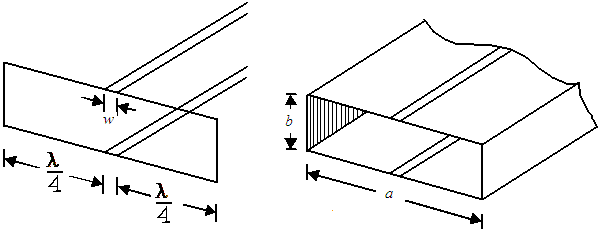
\includegraphics[width=6cm]{Cha6//fig6-0.png}
        \caption{从双导线到矩形波导}
    \end{figure}
\end{frame}

\subsection{预备知识}
\begin{frame}{预备知识}
    \begin{itemize}
        \item 交变电磁场基本关系式
    \end{itemize}
    \begin{align*}
        \begin{cases}
            \nabla\times\vec{E}=-\dfrac{\partial \vec{B}}{\partial t}        \\
            \nabla\times\vec{H}=\dfrac{\partial \vec{D}}{\partial t}+\vec{J} \\
            \nabla\cdot\vec{D}=\rho                                          \\
            \nabla\cdot\vec{B}=0
        \end{cases}
    \end{align*}
    \begin{align*}
        \vec{D}=\epsilon\vec{E},\vec{B}=\mu\vec{H},\vec{J}=\sigma\vec{E}
    \end{align*}
    无源区,时谐场
    \begin{align*}
        \begin{cases}
            \nabla\times\vec{E}=-\mathrm{j}\omega\mu\vec{H}     \\
            \nabla\times\vec{H}=\mathrm{j}\omega\epsilon\vec{E} \\
            \nabla\cdot\vec{D}=0                                \\
            \nabla\cdot\vec{B}=0
        \end{cases}
    \end{align*}
\end{frame}

\begin{frame}{预备知识}
    \begin{itemize}
        \item 边界条件
    \end{itemize}
    \begin{columns}
        \begin{column}{0.5\linewidth}
            两种媒质界面的边界条件
            \begin{align*}
                \begin{cases}
                    \hat{n}\times(\vec{E}_2-\vec{E}_1)=0         \\
                    \hat{n}\times(\vec{H}_2-\vec{H}_1)=\vec{J}_s \\
                    \hat{n}\cdot(\vec{D}_2-\vec{D}_1)=\rho_s     \\
                    \hat{n}\cdot(\vec{B}_2-\vec{B}_1)=0
                \end{cases}
            \end{align*}
        \end{column}
        \begin{column}{0.5\linewidth}
            理想导体表面的边界条件
            \begin{align*}
                \begin{cases}
                    \hat{n}\times\vec{E}_2=0         \\
                    \hat{n}\times\vec{H}_2=\vec{J}_s \\
                    \hat{n}\cdot\vec{D}_2=\rho_s     \\
                    \hat{n}\cdot\vec{B}_2=0
                \end{cases}
            \end{align*}
        \end{column}
    \end{columns}
\end{frame}

\begin{frame}
    \begin{itemize}
        \item 交变电磁场的能量关系
    \end{itemize}
    对于一封闭曲面S,电磁场的能量关系满足复功率定理,即
    \begin{align*}
        -\oint_S\frac{1}{2}(\vec{E}\times\vec{H}^*)\bullet\hat{n}\rm{d}S=P_L+\rm{j}2\omega(W_m-W_e)
    \end{align*}
\end{frame}

\begin{frame}{预备知识}
    \begin{itemize}
        \item 导波系统波型\\
              导波系统中的电磁波按纵向场分量的有无,分为以下三种波型(模)
              \begin{itemize}
                  \item 横磁波(TM波),又称电波(E波): $H_z=0,E_z\neq 0$
                  \item 横电波(TE波),又称磁波(H波): $E_z=0,H_z\neq 0$
                  \item 横电磁波(TEM波): $E_z=0,H_z=0$
              \end{itemize}
    \end{itemize}
\end{frame}

\begin{frame}{预备知识}
    \begin{itemize}
        \item 波导一般解的出发点和假定条件\\
              波导一般解的出发点是频域Maxwell方程组
              \begin{align}
                  \begin{cases}
                      \nabla\times\vec{H}=\mathrm{j}\omega\epsilon\vec{E} \\
                      \nabla\times\vec{E}=-\mathrm{j}\omega\mu\vec{H}     \\
                      \nabla\cdot\vec{E}=0                                \\
                      \nabla\cdot\vec{H}=0
                  \end{cases}
                  \label{eqn6-1}
              \end{align}
              波导假定条件
              \begin{columns}
                  \begin{column}{0.5\linewidth}
                      \begin{itemize}
                          \item 波导均匀条件:假定横截面不随$z$而变化
                          \item 媒质均匀条件:波导内部$\epsilon,\mu$均匀,波导内壁$\sigma$无限大
                          \item 无源条件:波导内$\rho,\vec{J}\equiv 0$
                          \item 无限条件:波导在$z$方向无限长
                      \end{itemize}
                  \end{column}
                  \begin{column}{0.5\linewidth}
                      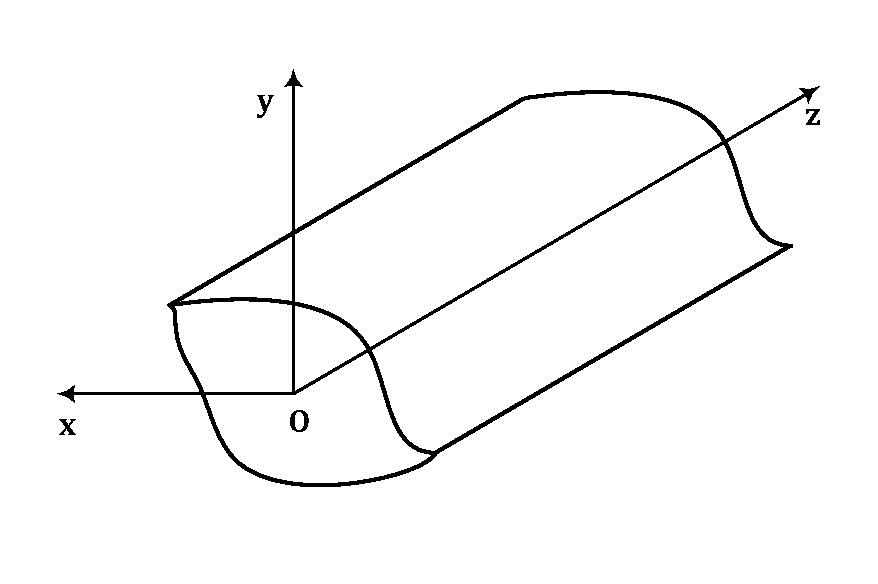
\includegraphics[width=5cm]{Cha6//fig6-1.pdf}
                  \end{column}
              \end{columns}
    \end{itemize}
\end{frame}

\subsection{矩形波导}

\begin{frame}{矩形波导——导模}
    \begin{itemize}
        \item 矩形波导的一般解
    \end{itemize}
    (\ref{eqn6-1})第二式两边取旋度
    \begin{align*}
        \nabla\times\nabla\times\vec{E} & =\nabla(\nabla\cdot\vec{E})-\nabla^2\vec{E}=-\mathrm{j}\omega\mu\nabla\times\vec{H} \\
                                        & =\omega^2\mu\epsilon\vec{E}=k^2\vec{E}                                              \\
                                        & k=\omega\sqrt{\mu\epsilon}=2\pi/\lambda
    \end{align*}
    得到波动方程
    \begin{align}
        \begin{cases}
            \nabla^2\vec{E}+k^2\vec{E}=0 \\
            \nabla^2\vec{H}+k^2\vec{H}=0 \\
        \end{cases}\label{eqn6-2}
    \end{align}
\end{frame}

\begin{frame}{矩形波导——导模}
    \begin{itemize}
        \item 纵向场表示横向场
    \end{itemize}
    \centering
    \begin{figure}
        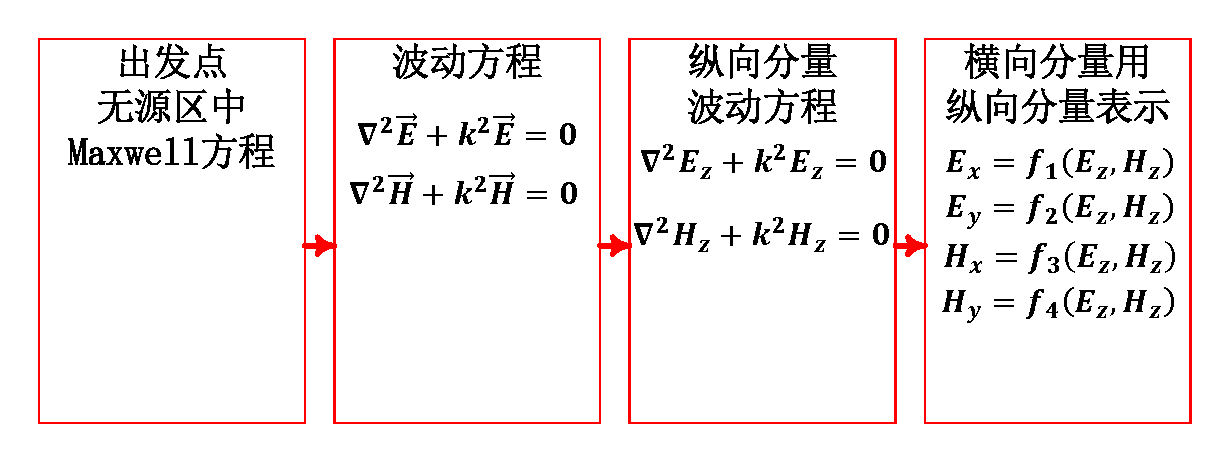
\includegraphics[width=10cm]{Cha6/fig6-2.pdf}
        \caption{纵向分量法流程图}   %\numberwithin{figure}{section}
    \end{figure}
\end{frame}

\begin{frame}{矩形波导——导模}
    纵向分量方程
    \begin{align}
        \begin{cases}
            \nabla^2E_z+k^2E_z=0 \\
            \nabla^2H_z+k^2H_z=0
        \end{cases}
        \label{eqn6-3}
    \end{align}
    假定$E_z$或$H_z$可分离变量,即
    \begin{align}
        \begin{cases}
            E_z=E(x,y)Z(z) \\
            H_z=H(x,y)W(z)
        \end{cases}
        \label{eqn6-4}
    \end{align}
    且$Laplace$算子$\nabla^2$可分解为
    \begin{align}
        \nabla^2=\nabla_t^2+\frac{\partial^2}{\partial z^2}
        \label{eqn6-5}
    \end{align}
    将式(\ref{eqn6-4})、式(\ref{eqn6-5})代入式(\ref{eqn6-3})可知
\end{frame}

\begin{frame}{矩形波导——导模}
    \begin{align}
        \frac{\nabla^2_t E(x,y)}{E(x,y)}+\frac{1}{Z(z)}\frac{\rm{d}^2 Z(z)}{\rm{d}z^2}+k^2=0
        \label{eqn6-6}
    \end{align}
    由于其独立性,上式各项均为常数
    \begin{align}
        \begin{cases}
            \dfrac{1}{Z(z)}\dfrac{\rm{d}Z(z)}{\rm{d}z^2}=\gamma^2 \\
            \dfrac{\nabla_t^2E(x,y)}{E(x,y)}+k_c^2=0
        \end{cases}
        \label{eqn6-7}
    \end{align}
    其中
    \begin{align}
        k_c^2=k^2+\gamma^2
    \end{align}
    称为\textbf{截止波数}
\end{frame}

\begin{frame}{矩形波导——导模}
    式(\ref{eqn6-7})中第一方程的解是
    \begin{align}
        Z(z)=C_1\rm{e}^{-\gamma z}+C_2\rm{e}^{\gamma z}
    \end{align}
    有趣的是:波导解的$z$函数与传输线解有惊人的相似,又是入射波和反射波的组合。我们只研究一个波(不论是TE或TM波),在形式上只写入射波
    \begin{align}
        \begin{cases}
            E_z=E(x,y)\rm{e}^{-\gamma z} \\
            H_z=H(x,y)\rm{e}^{-\gamma z}
        \end{cases}
    \end{align}
    $$\frac{\partial}{\partial z}\rightarrow -\gamma$$
\end{frame}

\begin{frame}{矩形波导——导模}
    \begin{align*}
        \nabla\times\vec{H}=\mathrm{j}\omega\epsilon \vec{E}
    \end{align*}
    \begin{align*}
         & \begin{vmatrix}
               \hat{x}                      & \hat{y}                      & \hat{z} \\
               \dfrac{\partial}{\partial x} & \dfrac{\partial}{\partial y} & -\gamma \\
               H_x                          & H_y                          & H_z     \\
           \end{vmatrix}
        =\rm{j}\omega\epsilon(\hat{x}E_x+\hat{y}E_y+\hat{z}E_z)
    \end{align*}
    \begin{align}
        \begin{cases}
            \dfrac{\partial H_z}{\partial y}+\gamma H_y=\rm{j}\omega\epsilon E_x  \\
            -\gamma H_x-\dfrac{\partial H_z}{\partial x}=\rm{j}\omega\epsilon E_y \\
            \dfrac{\partial H_y}{\partial x}-\dfrac{\partial H_x}{\partial y}=\rm{j}\omega\epsilon E_z
        \end{cases}
    \end{align}
\end{frame}

\begin{frame}{矩形波导——导模}
    \begin{align*}
        \nabla\times\vec{E}=-\mathrm{j}\omega\mu \vec{H}
    \end{align*}
    \begin{align*}
        \begin{vmatrix}
            \hat{x}                      & \hat{y}                      & \hat{z} \\
            \dfrac{\partial}{\partial x} & \dfrac{\partial}{\partial y} & -\gamma \\
            E_x                          & E_y                          & E_z     \\
        \end{vmatrix}
        =-\rm{j}\omega\mu(\hat{x}H_x+\hat{y}H_y+\hat{z}H_z)
    \end{align*}
    \begin{align}
        \begin{cases}
            \dfrac{\partial E_z}{\partial y}+\gamma E_y=-\rm{j}\omega\mu H_x  \\
            -\gamma E_x-\dfrac{\partial E_z}{\partial x}=-\rm{j}\omega\mu H_y \\
            \dfrac{\partial E_y}{\partial x}-\dfrac{\partial E_x}{\partial y}=-\rm{j}\omega\mu H_z
        \end{cases}
    \end{align}
\end{frame}

\begin{frame}{矩形波导——导模}
    先整理$E_x,H_y$方程组,得
    \begin{align*}
        \begin{cases}
            \rm{j}\omega\epsilon E_x-\gamma H_y=\dfrac{\partial H_z}{\partial y} \\
            -\gamma E_x+\rm{j}\omega\mu H_y=\dfrac{\partial E_z}{\partial x}     \\
        \end{cases}
    \end{align*}
    \begin{align*}
        D=
        \begin{vmatrix}
            \rm{j}\omega\epsilon & -\gamma         \\
            -\gamma              & \rm{j}\omega\mu \\
        \end{vmatrix}
        =-k^2-\gamma^2=-k_c^2
    \end{align*}
    \begin{align*}
        D_x=
        \begin{vmatrix}
            \dfrac{\partial H_z}{\partial y} & -\gamma         \\
            \dfrac{\partial E_z}{\partial x} & \rm{j}\omega\mu \\
        \end{vmatrix}
        =\gamma\frac{\partial E_z}{\partial x}+\rm{j}\omega\mu\frac{\partial H_z}{\partial y}
    \end{align*}
    \begin{align*}
        D_y=
        \begin{vmatrix}
            \rm{j}\omega\epsilon & \dfrac{\partial H_z}{\partial y} \\
            -\gamma              & \dfrac{\partial E_z}{\partial x} \\
        \end{vmatrix}
        =\rm{j}\omega\epsilon\frac{\partial E_z}{\partial x}+\gamma \frac{\partial H_z}{\partial y}
    \end{align*}
\end{frame}

\begin{frame}{矩形波导——导模}
    \begin{align}
        \begin{cases}
            E_x=\dfrac{D_x}{D}=-\dfrac{1}{k_c^2}\left(\gamma\dfrac{\partial E_z}{\partial x}+\rm{j}\omega\mu\dfrac{\partial H_z}{\partial y}\right) \\
            H_y=\dfrac{D_y}{D}=-\dfrac{1}{k_c^2}\left(\rm{j}\omega\epsilon\dfrac{\partial E_z}{\partial x}+\gamma\dfrac{\partial H_z}{\partial y}\right)
        \end{cases}
        \label{eqn6-13}
    \end{align}
\end{frame}

\begin{frame}{矩形波导——导模}
    再整理$E_y,H_x$方程组,得
    \begin{align*}
        \begin{cases}
            \rm{j}\omega\epsilon E_y+\gamma H_x=-\dfrac{\partial H_z}{\partial x} \\
            \gamma E_y+\rm{j}\omega\mu H_x=-\dfrac{\partial E_z}{\partial y}
        \end{cases}
    \end{align*}
    \begin{align*}
        D=
        \begin{vmatrix}
            \rm{j}\omega\epsilon & \gamma          \\
            \gamma               & \rm{j}\omega\mu \\
        \end{vmatrix}
        =-k^2-\gamma^2=-k_c^2
    \end{align*}
    \begin{align*}
        D_y=
        \begin{vmatrix}
            -\dfrac{\partial H_z}{\partial x} & \gamma          \\
            -\dfrac{\partial E_z}{\partial y} & \rm{j}\omega\mu \\
        \end{vmatrix}
        =\gamma\frac{\partial E_z}{\partial y}-\rm{j}\omega\mu\frac{\partial H_z}{\partial x}
    \end{align*}
    \begin{align*}
        D_x=
        \begin{vmatrix}
            \rm{j}\omega\epsilon & -\dfrac{\partial H_z}{\partial x} \\
            \gamma               & -\dfrac{\partial E_z}{\partial y} \\
        \end{vmatrix}
        =-\rm{j}\omega\epsilon\frac{\partial E_z}{\partial y}+\gamma \frac{\partial H_z}{\partial x}
    \end{align*}
\end{frame}

\begin{frame}{矩形波导——导模}
    \begin{align}
        \begin{cases}
            E_y=\dfrac{D_y}{D}=\dfrac{1}{k_c^2}\left(-\gamma\dfrac{\partial E_z}{\partial y}+\rm{j}\omega\mu\dfrac{\partial H_z}{\partial x}\right) \\
            H_x=\dfrac{D_x}{D}=\dfrac{1}{k_c^2}\left(\rm{j}\omega\epsilon\dfrac{\partial E_z}{\partial y}-\gamma\dfrac{\partial H_z}{\partial x}\right)
        \end{cases}
        \label{eqn6-14}
    \end{align}
    把(\ref{eqn6-13})和(\ref{eqn6-14})进一步归纳成矩阵形式,得
    \begin{empheq}[box=\widefbox]{align}
        \begin{bmatrix}
            E_x \\
            E_y \\
            H_x \\
            H_y \\
        \end{bmatrix}
        =\frac{1}{k_c^2}
        \begin{bmatrix}
            -\gamma               & 0                    & 0               & -\rm{j}\omega\mu \\
            0                     & -\gamma              & \rm{j}\omega\mu & 0                \\
            0                     & \rm{j}\omega\epsilon & -\gamma         & 0                \\
            -\rm{j}\omega\epsilon & 0                    & 0               & -\gamma          \\
        \end{bmatrix}
        \begin{bmatrix}
            \dfrac{\partial E_z}{\partial x} \\
            \dfrac{\partial E_z}{\partial y} \\
            \dfrac{\partial H_z}{\partial x} \\
            \dfrac{\partial H_z}{\partial y} \\
        \end{bmatrix}
    \end{empheq}
    $$\epsilon=\epsilon_0\epsilon_r(1-\rm{j}\tan\delta)$$
    $$\text{损耗角正切:} \tan\delta=\sigma/\omega\epsilon_0\epsilon_r$$
\end{frame}

\begin{frame}{矩形波导——TE模}
    \begin{itemize}
        \item 矩形波导的横向解
    \end{itemize}
    在矩形波导中存在TE和TM两类模,这里以TE模为例进行讨论,即$E_z=0$,对于纵向分量只需讨论$H_z$
    \begin{columns}
        \begin{column}{0.4\linewidth}
            \begin{align*}
                \nabla_t^2=\frac{\partial^2}{\partial x^2}+\frac{\partial^2}{\partial y^2} \\
                \frac{\nabla_t^2H_z(x,y)}{H_z(x,y)}+k_c^2=0
            \end{align*}
        \end{column}
        \begin{column}{0.6\linewidth}
            \begin{figure}
                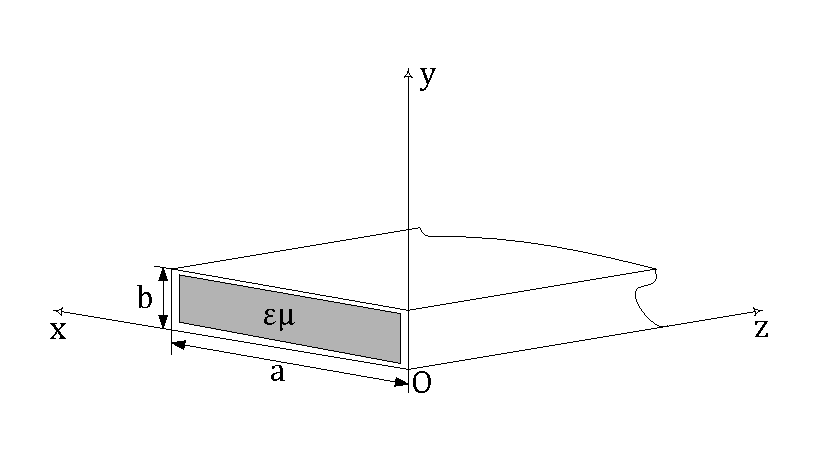
\includegraphics[width=7cm]{Cha6//fig6-3.pdf}
                \caption{矩形波导坐标系}
            \end{figure}
        \end{column}
    \end{columns}
\end{frame}

\begin{frame}{矩形波导——TE模}
    \begin{align}
        \frac{\partial^2H_z(x,y)}{\partial x^2}+\frac{\partial^2H_z(x,y)}{\partial y^2}=-k_c^2H_z(x,y)
        \label{eqn6-16}
    \end{align}
    $H_z(x,y)$可分离变量,即$H_z(x,y)=X(x)Y(y)$,(\ref{eqn6-16})可写为
    \begin{align}
        \frac{1}{X}\frac{\rm{d}^2X}{\rm{d}x^2}+\frac{1}{Y}\frac{\rm{d}^2Y}{\rm{d}y^2}=-k_c^2
        \label{eqn6-17}
    \end{align}
    式(\ref{eqn6-17})左边每项都是常数,可得
    \begin{align}
        \begin{cases}
            \dfrac{1}{X}\dfrac{\rm{d}^2X}{\rm{d}x^2}=-k_x^2 \\
            \dfrac{1}{Y}\dfrac{\rm{d}^2Y}{\rm{d}y^2}=-k_y^2 \\
            k_x^2+k_y^2=k_c^2
        \end{cases}
    \end{align}
    一般解为
    \begin{align*}
        X=A\cos(k_x x+\varphi_x);Y=B\cos(k_y y+\varphi_y)
    \end{align*}

\end{frame}

\begin{frame}{矩形波导——TE模}
    总的纵向磁场为:
    \begin{align}
        H_z=H_0\cos(k_x x+\varphi_x)\cos(k_y y+\varphi_y)\rm{e}^{-\gamma z}
    \end{align}
    $H_0$在问题中认为是未知数,与具体激励强度有关。
    \begin{align*}
        \begin{cases}
            E_x = -\dfrac{\rm{j}\omega\mu}{k_c^2}\dfrac{\partial H_z}{\partial y}=H_0\dfrac{\rm{j}\omega\mu}{k_c^2}k_y\cos(k_x x+\varphi_x)\sin(k_y y+\varphi_y)\rm{e}^{-\gamma z} \\
            E_y = \dfrac{\rm{j}\omega\mu}{k_c^2}\dfrac{\partial H_z}{\partial x}=-H_0\dfrac{\rm{j}\omega\mu}{k_c^2}k_x\sin(k_x x+\varphi_x)\cos(k_y y+\varphi_y)\rm{e}^{-\gamma z}
        \end{cases}
    \end{align*}
    利用边界条件,即波导4个边壁上电场切向分量为0
    \begin{align*}
        \begin{cases}
            E_y = 0 \qquad x=0,x=a \\
            E_x = 0 \qquad y=0,y=b
        \end{cases}
    \end{align*}
\end{frame}

\begin{frame}{矩形波导——TE模}
    \begin{align*}
        \begin{cases}
            x=0,E_y=0 \rightarrow \varphi_x=0                                              \\
            x=a,E_y=0 \rightarrow k_x a=m\pi \rightarrow k_x=\frac{m\pi}{a},m=0,1,2,\cdots \\
            y=0,E_x=0 \rightarrow \varphi_y=0                                              \\
            y=b,E_x=0 \rightarrow k_y b=n\pi \rightarrow k_y=\frac{n\pi}{b},n=0,1,2,\cdots
        \end{cases}
    \end{align*}
    \begin{align}
        \begin{cases}
            H_z=H_0\cos\left(\dfrac{m\pi}{a}x\right)\cos\left(\dfrac{n\pi}{b}y\right)\rm{e}^{-\gamma z}                                               \\
            E_x=\rm{j}\dfrac{\omega\mu}{k_c^2}\dfrac{n\pi}{b}H_0\cos\left(\dfrac{m\pi}{a}x\right)\sin\left(\dfrac{n\pi}{b}y\right)\rm{e}^{-\gamma z}  \\
            E_y=-\rm{j}\dfrac{\omega\mu}{k_c^2}\dfrac{m\pi}{a}H_0\sin\left(\dfrac{m\pi}{a}x\right)\cos\left(\dfrac{n\pi}{b}y\right)\rm{e}^{-\gamma z} \\
            E_z=0                                                                                                                                     \\
            H_x=\dfrac{\gamma}{k_c^2}\dfrac{m\pi}{a}H_0\sin\left(\dfrac{m\pi}{a}x\right)\cos\left(\dfrac{n\pi}{b}y\right)\rm{e}^{-\gamma z}           \\
            H_y=\dfrac{\gamma}{k_c^2}\dfrac{n\pi}{b}H_0\cos\left(\dfrac{m\pi}{a}x\right)\sin\left(\dfrac{n\pi}{b}y\right)\rm{e}^{-\gamma z}
        \end{cases}
    \end{align}

\end{frame}

\begin{frame}{矩形波导——TE模}
    \begin{align}
        k_c^2=k_x^2+k_y^2=\left(\frac{m\pi}{a}\right)^2+\left(\frac{n\pi}{b}\right)^2
    \end{align}
    上述$TE$模称为$TE_{mn}$模,其中$m$表示$x$方向变化的半周期数;$n$表示$y$方向变化的半周期数。由于$m=0$及$n=0$时所有场分量才为0,因此
    矩形波导中存在$TE_{m0}$和$TE_{0n}$等波形。若$a>b$,则模$TE_{10}$是最低次波型,其余波型为高次波型。\\
    关于\textbf{本征模}:\\
    以矩形波导为例,尽管在$z$方向它们只可能是入射波加反射波,但是由于横向边界条件的约束,它们由$TE_{mn}$
    和$TM_{mn}$模组成,并且只能由$TE_{mn}$和$TM_{mn}$模组成(后者称为完备性),矩形波导中这些模的完备
    集合就是本征模。
\end{frame}

\begin{frame}{矩形波导——TM模}
    同理,对于$TM$模来说$H_z=0$总的纵向电场为:
    \begin{align}
        E_z=E_0\sin\left(\frac{m\pi}{a}x\right)\sin\left(\frac{n\pi}{b}y\right)\rm{e}^{-\gamma z}
    \end{align}
    本征值:
    $$k_x=\frac{m\pi}{a},k_y=\frac{n\pi}{b}\quad m,n=1,2,\cdots$$

    \begin{align*}
        \begin{cases}
            E_x = -\rm{j}\dfrac{\beta}{k_c^2}\left(\dfrac{m\pi}{a}\right)E_0\cos\left(\dfrac{m\pi}{a}x\right)\sin\left(\dfrac{n\pi}{b}y\right)\rm{e}^{-\gamma z}          \\
            E_y = -\rm{j}\dfrac{\beta}{k_c^2}\left(\dfrac{n\pi}{b}\right)E_0\sin\left(\dfrac{m\pi}{a}x\right)\cos\left(\dfrac{n\pi}{b}y\right)\rm{e}^{-\gamma z}          \\
            H_x = \rm{j}\dfrac{\omega\epsilon}{k_c^2}\left(\dfrac{n\pi}{b}\right)E_0\sin\left(\dfrac{m\pi}{a}x\right)\cos\left(\dfrac{n\pi}{b}y\right)\rm{e}^{-\gamma z}  \\
            H_y = -\rm{j}\dfrac{\omega\epsilon}{k_c^2}\left(\dfrac{m\pi}{a}\right)E_0\cos\left(\dfrac{m\pi}{a}x\right)\sin\left(\dfrac{n\pi}{b}y\right)\rm{e}^{-\gamma z} \\
            H_z = 0
        \end{cases}
    \end{align*}
\end{frame}

\begin{frame}{矩形波导——TM模}
    上述$TM$模称为$TM_{mn}$模,其中$m$表示$x$方向变化的半周期数;$n$表示$y$方向变化的半周期数。由于$m=0$或$n=0$时所有场分量均为0,因此
    矩形波导中不存在$TM_{00}$、$TM_{0n}$及$TM_{m0}$等波形。所以$TM_{11}$是最低次波型,其余波型为高次波型。\\
\end{frame}

\begin{frame}{矩形波导-场结构}
    \begin{itemize}
        \item $TE_{10}模$
    \end{itemize}
    即$TE_{mn}$模中下标$m=1,n=0$的情况,是满足$a>b$条件下的矩形波导中\textbf{截止频率}最低的模式,也叫主模。
    \begin{align*}
        \begin{cases}
            H_z=H_0\cos\left(\dfrac{\pi}{a}x\right)\rm{e}^{-\rm{j}\beta z}                                                           \\
            E_y=-\rm{j}\dfrac{\omega\mu}{k_c^2}\left(\dfrac{\pi}{a}\right)H_0\sin\left(\dfrac{\pi}{a}x\right)\rm{e}^{-\rm{j}\beta z} \\
            H_x=\dfrac{\rm{j}\beta}{k_c^2}\left(\dfrac{\pi}{a}\right)H_0\sin\left(\dfrac{\pi}{a}x\right)\rm{e}^{-\rm{j}\beta z}
        \end{cases}
    \end{align*}
    只取其实部解,得
    \begin{align*}
        \begin{cases}
            H_z=H_0\cos\left(\dfrac{\pi}{a}x\right)\cos(\omega t-\beta z)                                                    \\
            E_y=\dfrac{\omega\mu}{k_c^2}\left(\dfrac{\pi}{a}\right)H_0\sin\left(\dfrac{\pi}{a}x\right)\sin(\omega t-\beta z) \\
            H_x=-\dfrac{\beta}{k_c^2}\left(\dfrac{\pi}{a}\right)H_0\sin\left(\dfrac{\pi}{a}x\right)\sin(\omega t-\beta z)
        \end{cases}
    \end{align*}
\end{frame}

\begin{frame}{矩形波导——场结构}
    \begin{itemize}
        \item $TE_{10}$模场结构
    \end{itemize}
    $TE_{10}$模场强与$y$无关,场分量沿$y$轴均匀分布。沿$x$轴的变化规律为:
    $$E_y \propto \sin(\pi x/a),H_x \propto \sin(\pi x/a),H_z \propto \cos(\pi x/a)$$
    \begin{columns}
        \begin{column}{0.7\linewidth}
            \begin{figure}
                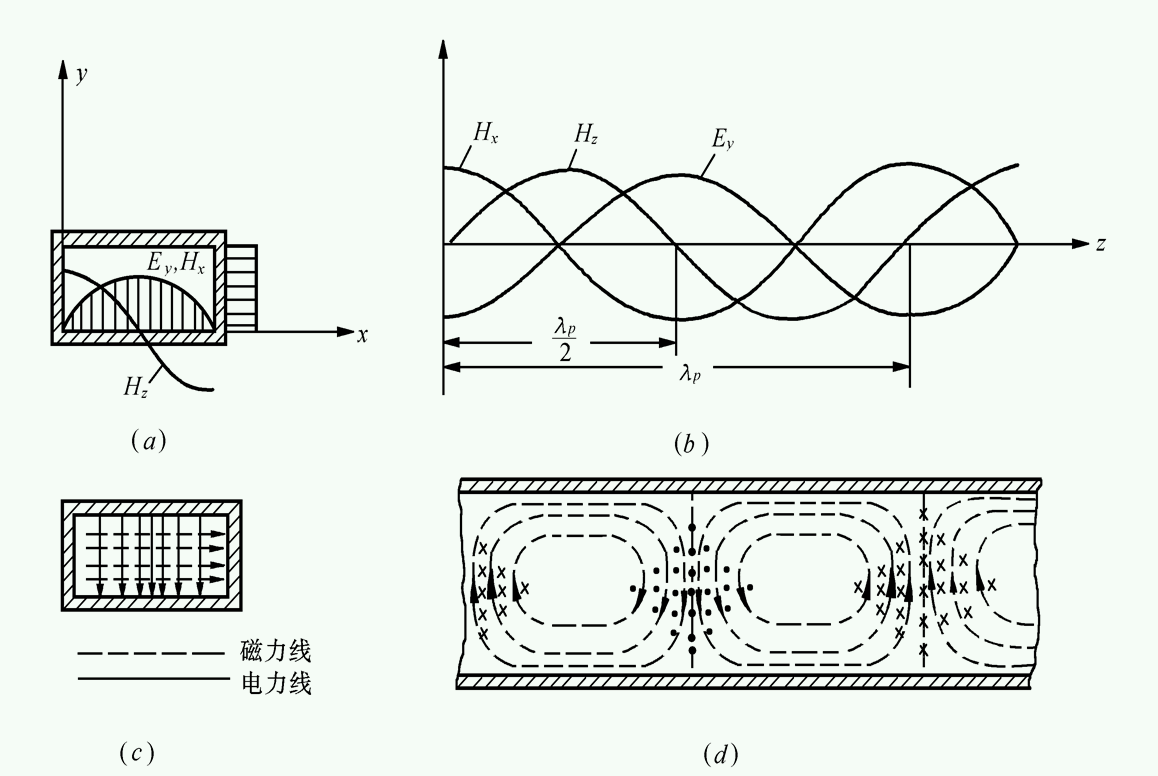
\includegraphics[width=7cm]{Cha6//fig6-4.png}
                \caption{\footnotesize{矩形波导$TE_{10}$模场分量分布规律}}
            \end{figure}
        \end{column}
        \begin{column}{0.3\linewidth}
            {\footnotesize (a)场分量沿$x$轴变化规律\\
                (b)场分量沿$z$轴变化规律\\
                (c)矩形波导横截面场分布\\
                (d)矩形波导纵剖面场分布}
        \end{column}
    \end{columns}
\end{frame}

\begin{frame}{矩形波导——场结构}
    某一时刻$TE_{10}$模完整的场分布,随时间推移,场分布图以相速$v_P$沿传输方向移动
    \begin{figure}
        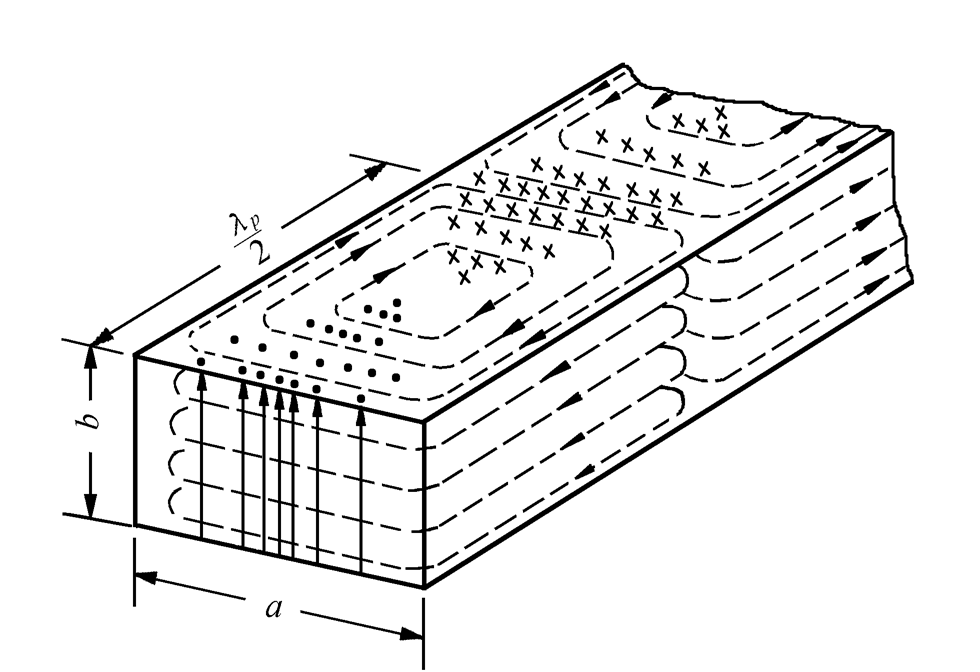
\includegraphics[width=9cm]{Cha6//fig6-5.png}
        \caption{\footnotesize{矩形波导$TE_{10}$模场分布图}}
    \end{figure}
\end{frame}

\begin{frame}{矩形波导——管壁电流}
    \begin{itemize}
        \item 根据导体中电磁波传播,在微波波段,趋肤效应使感应电流在很薄的波导内壁表面流动  ————称为\textbf{壁电流}
    \end{itemize}
    \begin{columns}
        \begin{column}{0.5\linewidth}
            $$\vec{J_S}=\hat{n}\times\vec{H}_{\tan}$$
        \end{column}
        \begin{column}{0.5\linewidth}
            \begin{figure}
                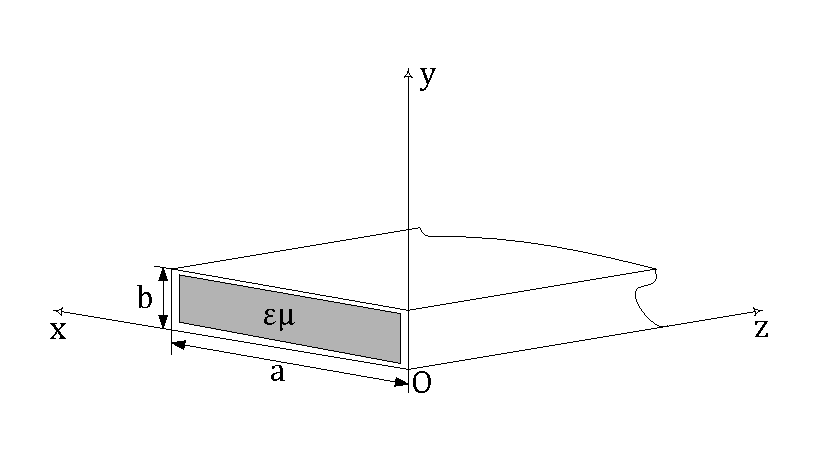
\includegraphics[width=5cm]{Cha6//fig6-3.pdf}
            \end{figure}
        \end{column}
    \end{columns}
    以$TE_{10}$模为例
    \begin{align*}
        \begin{cases}
            \vec{J_S}|_{y=0}=\hat{y}\times[\hat{x}H_x+\hat{z}H_z]_{y=0}=[\hat{x}H_z-\hat{z}H_x]_{y=0}   \\
            \vec{J_S}|_{y=b}=-\hat{y}\times[\hat{x}H_x+\hat{z}H_z]_{y=b}=[-\hat{x}H_z+\hat{z}H_x]_{y=b} \\
            \vec{J_S}|_{x=0}=\hat{x}\times\hat{z}H_z|_{x=0}=-\hat{y}H_z|_{x=0}                          \\
            \vec{J_S}|_{x=a}=-\hat{x}\times\hat{z}H_z|_{x=a}=\hat{y}H_z|_{x=a}
        \end{cases}
    \end{align*}
\end{frame}

\begin{frame}{矩形波导——管壁电流}
    \begin{align*}
        \color{blue}{\vec{J_S}(y=0)=[\hat{x}H_{10}\cos(\pi x/a)-\mathrm{j}\hat{z}\frac{\beta a}{\pi}H_{10}\sin(\pi x/a)]} \\
        \color{blue}{\vec{J_S}(y=b)=[-\hat{x}H_{10}\cos(\pi x/a)+\mathrm{j}\hat{z}\frac{\beta a}{\pi}H_{10}\sin(\pi x/a)]}
    \end{align*}
    \begin{columns}
        \begin{column}{0.5\linewidth}
            \begin{figure}
                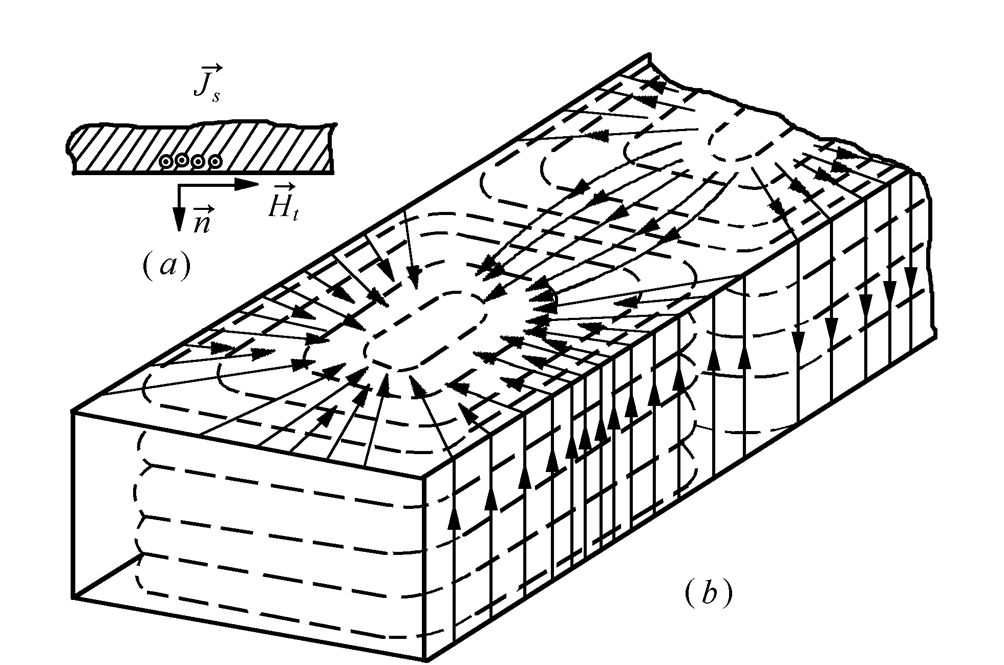
\includegraphics[width=6cm]{Cha6//fig6-6.png}
                \caption{矩形波导$TE_{10}$模管壁电流分布}
            \end{figure}
        \end{column}
        \begin{column}{0.5\linewidth}
            \fbox{面电流与磁力线、表面法向正交}
            \begin{align*}
                \vec{J_S}(x=0)=-\hat{y}H_{10} \\
                \vec{J_S}(x=a)=-\hat{y}H_{10}
            \end{align*}
        \end{column}
    \end{columns}
\end{frame}

\begin{frame}{矩形波导——管壁电流}
    中间的源由场的变化——也即位移电流$\frac{\partial\vec{D}}{\partial t}$形成的。\\
    \hspace*{\fill}\\
    在波导中凡是\textbf{切割电流}都要引起辐射和损耗,如图\ref{fig6-7png}所示,所以波导与波导连接时一定要处理好。
    \begin{figure}
        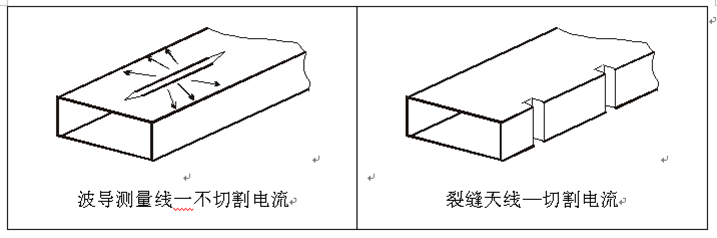
\includegraphics[width=8cm]{Cha6//fig6-7.png}
        \caption{不切割电流和切割电流的波导}
        \label{fig6-7png}
    \end{figure}
\end{frame}

\begin{frame}{矩形波导——传输特性}
    \begin{itemize}
        \item 截止特性
    \end{itemize}
    由于$k_c^2=k^2+\gamma^2=k^2-\beta^2=\left(\frac{m\pi}{a}\right)^2+\left(\frac{n\pi}{b}\right)^2$,
    而传播相位因子$\rm{e}^{-\rm{j}\beta z}$中,如$\beta$需要是实数,必须满足
    $$\beta^2=k^2-k_c^2>0或k>k_c$$
    对于$TE_{10}$模来说,必须要满足
    \begin{align}
        \frac{2\pi}{\lambda}>\frac{\pi}{a}\qquad \lambda<2a
    \end{align}
    为此,定义
    \begin{align}
        k_c=\frac{2\pi}{\lambda_c}
    \end{align}
    其中,$\lambda_c=2a$称为截止波长;$k_c$是对应的截止波数。
\end{frame}

\begin{frame}{矩形波导——传输特性}
    TE波和TM波的\textbf{截止频率}为
    \begin{align*}
        f_c=\frac{v}{\lambda_c}=\frac{k_c}{2\pi\sqrt{\mu\epsilon}}=\frac{1}{2\sqrt{\mu\epsilon}}\sqrt{\left(\frac{m}{a}\right)^2+\left(\frac{n}{b}\right)^2}
    \end{align*}
    截止波长:
    \begin{empheq}[box=\fbox]{align*}
        \lambda_c=\frac{2\pi}{k_c}=\frac{2}{\sqrt{(m/a)^2+(n/b)^2}}
    \end{empheq}
    截止条件可记为:
    $$f<f_c或\lambda>\lambda_c$$\\
    截止波长不仅与波导尺寸$a$和$b$有关,而且与决定波型的$m$和$n$有关,截止频率还与介质特性有关。在这种意义下,波导是一个\textcolor{blue}{高通}滤波器,“低频”信号无法通过。
\end{frame}

\begin{frame}{矩形波导——传输特性}
    当波导尺寸$a$和$b$给定时,将不同$m$和$n$值代入,即可得到不同波型的截止波长。其分布如图
    \begin{figure}
        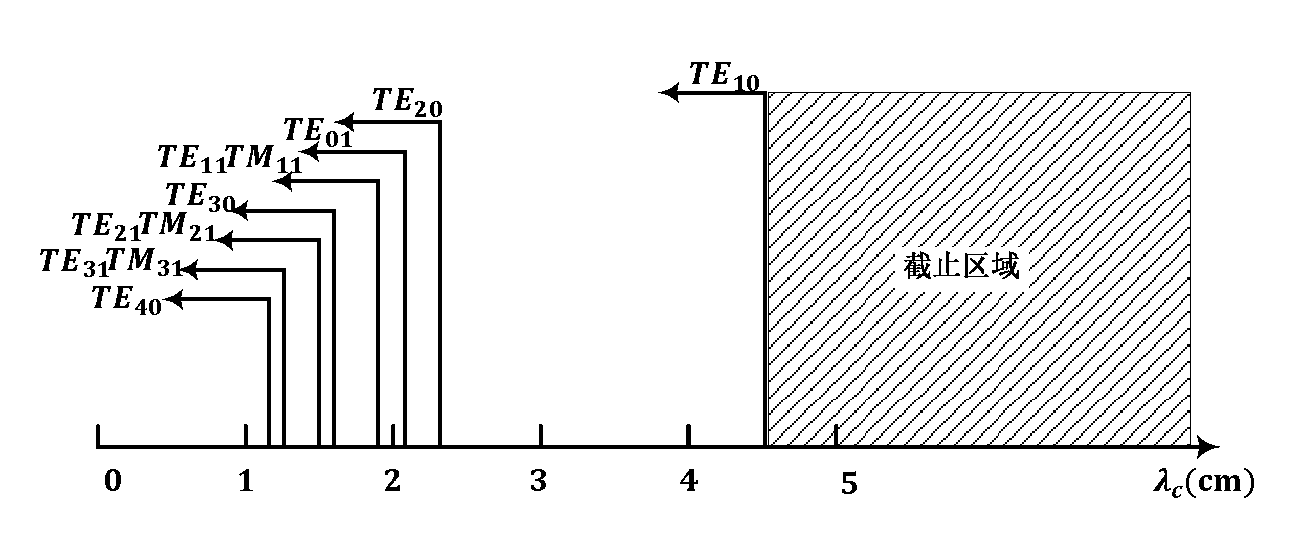
\includegraphics[width=8cm]{Cha6//fig6-7.pdf}
        \caption{BJ-100型波导不同波型截止波长分布图}
    \end{figure}
    从图中可以看到,$TE_{10}$模的截止波长最长,右边的阴影区为截止区。
\end{frame}

\begin{frame}{矩形波导——传输特性}
    \begin{itemize}
        \item 模式简并
    \end{itemize}
    不同导模的截止波长$\lambda_c$相同现象\\
    相同的波型指数$m$和$n$的$TE_{mn}$和$TM_{mn}$的截止波长相同,矩形波导的导模具有双重简并。
    \begin{itemize}
        \item 主模$TE_{10}$模——主模
              \begin{enumerate}
                  \item 通常矩形波导工作在$TE_{10}$单模传输情况,因为$TE_{10}$模容易实现单模传输。
                  \item 当工作频率一定时传输$TE_{10}$模的波导尺寸最小
                  \item 若波导尺寸一定,则实现单模传输的频带最宽。
              \end{enumerate}
    \end{itemize}
    为了实现$TE_{10}$单模传输,则要求电磁波的工作波长必须满足下列条件
    \begin{align*}
        \begin{cases}
            \lambda_c(TE_{20})<\lambda<\lambda_c(TE_{10}) \\
            \lambda>\lambda_c(TE_{01})
        \end{cases}
        \rightarrow
        \begin{cases}
            a<\lambda<2a \\
            \lambda>2b
        \end{cases}
    \end{align*}
    当工作波长给定时,若要实现$TE_{10}$单模传输,则波导尺寸必须满足
    $$\lambda/2<a<\lambda \quad b<\lambda/2$$
\end{frame}

\begin{frame}{矩形波导——传输特性}
    \begin{itemize}
        \item 波导波长$\lambda_g$
    \end{itemize}
    \begin{align}
        \lambda_g=\frac{\lambda}{\sqrt{1-\left(\frac{\lambda}{\lambda_c}\right)^2}}
    \end{align}
    很明显,波导波长$\lambda_g$大于自由空间波长$\lambda$。设传播常数$\beta=\dfrac{2\pi}{\lambda_g}$,则有
    $$\beta^2=k^2-k_c^2=\left(\frac{2\pi}{\lambda}\right)^2-\left(\frac{2\pi}{\lambda_c}\right)^2=\left(\frac{2\pi}{\lambda_g}\right)^2$$
    即可推导得
    $$\lambda_g=\frac{\lambda}{\sqrt{1-\left(\frac{\lambda}{\lambda_c}\right)^2}}=\frac{\lambda}{\sqrt{1-\left(\frac{\lambda}{2a}\right)^2}}$$
\end{frame}

\begin{frame}{矩形波导——传输特性}
    \begin{itemize}
        \item 相速$v_p$
    \end{itemize}
    \begin{align}
        v_p=\frac{c}{\sqrt{1-\left(\frac{\lambda}{\lambda_c}\right)^2}}=\frac{c}{\sqrt{1-\left(\frac{\lambda}{2a}\right)^2}}>c
    \end{align}
    已知相位因子构成的等相位面
    \begin{align*}
         & \omega t-\beta z=const                                                                                            \\
         & v_p=\frac{\rm{d}z}{\rm{d}t}=\frac{\omega}{\beta}=\frac{2\pi c/\lambda}{2\pi/\lambda_g}=c\frac{\lambda_g}{\lambda} \\
         & =\frac{c}{\sqrt{1-\left(\frac{\lambda}{\lambda_c}\right)^2}}=\frac{c}{\sqrt{1-\left(\frac{\lambda}{2a}\right)^2}}
    \end{align*}
    显然相速$v_p$大于自由空间光速,但相速并不是能量传播速度。
\end{frame}

\begin{frame}{矩形波导——传输特性}
    \begin{itemize}
        \item 群速$v_g$
    \end{itemize}
    \begin{align*}
        v_g                              & =\frac{\rm{d}\omega}{\rm{d}\beta}                                                                           \\
        \beta                            & = \sqrt{k^2-k_c^2}=\sqrt{\omega^2\epsilon\mu-k_c^2}                                                         \\
        \frac{\rm{d}\beta}{\rm{d}\omega} & =\frac{1}{2}\frac{2\omega\epsilon\mu}{\sqrt{k^2-k_c^2}}=\frac{k^2/\omega}{\sqrt{k^2-k_c^2}}=\frac{v_p}{c^2}
    \end{align*}
    \begin{align}
        v_g = \frac{c^2}{v_p}=c\sqrt{1-\left(\frac{\lambda}{\lambda_c}\right)^2}=c\sqrt{1-\left(\frac{\lambda}{2a}\right)^2}<c
    \end{align}
    \begin{align}
        v_p v_g=c^2
    \end{align}
\end{frame}

\begin{frame}{矩形波导——传输特性}
    \begin{itemize}
        \item 色散
    \end{itemize}
    TE波和TM波的相速和群速都随波长而变化,即是频率的函数,这种现象称为“\textbf{色散}”。因此,TE波和TM波统称为“色散波”;而TEM波
    的相速和群速相同,且与频率无关,没有色散现象,故称为“非色散波”。\\
    \hspace*{\fill} \\
    \textcolor{blue}{波导色散现象}与基于媒质特性产生的色散现象不同。由于我们已假定波导中媒质是线性的,即不随频率变化,所以波导中
    电磁波产生色散的原因是由\textcolor{blue}{波导系统本身的特性(边界条件)}所引起的。
\end{frame}

\begin{frame}{矩形波导——传输特性}
    \begin{itemize}
        \item 波型阻抗
    \end{itemize}
    $$Z=\frac{E_{u1}}{H_{u2}}=-\frac{E_{u2}}{H_{u1}}$$
    \begin{gather}
        Z_{TEM}=\frac{\omega\mu}{k}=\sqrt{\frac{\mu}{\epsilon}}=\eta\\
        Z_{TE}=\left|\frac{E_t}{H_t}\right|=\frac{\omega\mu}{\beta}=\sqrt{\frac{\mu}{\epsilon}}\frac{k}{\beta}=\eta\frac{\lambda_g}{\lambda}=\eta\frac{1}{\sqrt{1-\left(\frac{\lambda}{\lambda_c}\right)^2}}\\
        \color{blue}{Z_{TE_{10}}=\left|\frac{E_y}{H_x}\right|=\sqrt{\frac{\mu}{\epsilon}}\bullet\frac{1}{\sqrt{1-\left(\frac{\lambda}{2a}\right)^2}}}\\
        Z_{TM}=\left|\frac{E_t}{H_t}\right|=\frac{\beta}{\omega\epsilon}=\sqrt{\frac{\mu}{\epsilon}}\frac{\beta}{k}=\eta\sqrt{1-\left(\frac{\lambda}{\lambda_c}\right)^2}
    \end{gather}
\end{frame}

\begin{frame}{矩形波导——传输特性}
    \begin{itemize}
        \item $TE_{10}$模的功率和容量
    \end{itemize}
    \begin{figure}
        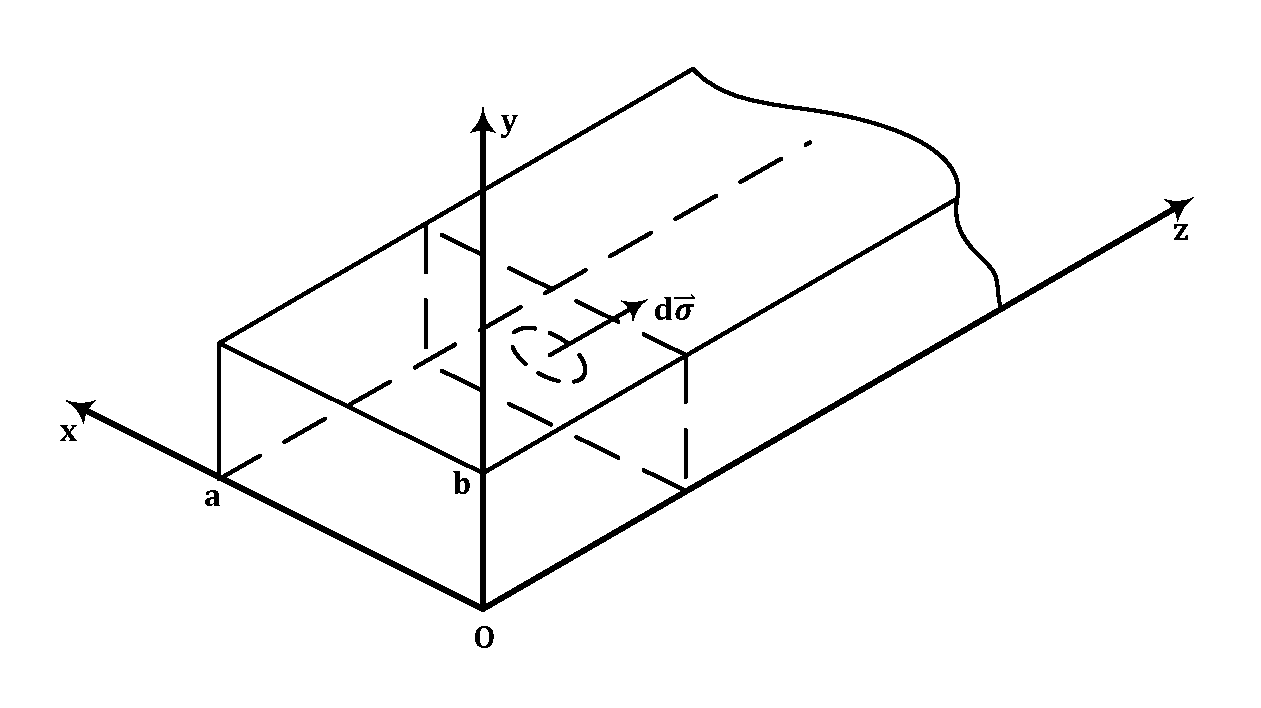
\includegraphics[width=8cm]{Cha6//fig6-8.pdf}
        \caption{计算功率时的面积元}
    \end{figure}
    \begin{align*}
        P=\iint_S\vec{S}\bullet\mathrm{d}\vec{\sigma}=\iint_S\frac{1}{2}\mathrm{Re}(\vec{E}_t\times\vec{H}_t^*)\bullet\hat{z}\mathrm{d}x\mathrm{d}y \\
        \vec{S}=\tfrac{1}{2}\mathrm{Re}(\vec{E}_t\times\vec{H}_t^*)\scriptsize{是Poynting矢量,}\mathrm{d}\vec{\sigma}\scriptsize{是面积元}
    \end{align*}
\end{frame}

\begin{frame}{矩形波导——传输特性}
    \begin{align*}
        \vec{S}\bullet\mathrm{d}\vec{\sigma} & =\frac{1}{2}\frac{E_0^2}{\eta}\sin^2\left(\frac{\pi}{a}x\right)\mathrm{d}x\mathrm{d}y                        \\
        P                                    & =\frac{1}{2}\frac{E_0^2}{\eta}\int_0^a\int_0^b\sin^2\left(\frac{\pi}{a}x\right)\mathrm{d}x\mathrm{d}y        \\
                                             & =\frac{1}{2}\frac{E_0^2}{\eta}b\int_0^a\frac{1}{2}\left[1-\cos\left(\frac{2\pi}{a}x\right)\right]\mathrm{d}x \\
                                             & =\frac{1}{4}\frac{E_0^2}{\eta}ab
    \end{align*}
    空气波导$\sqrt{\frac{\mu}{\epsilon}}=120\pi$,因此$P=\frac{E_0^2ab}{480\pi}\sqrt{1-\left(\frac{\lambda}{2a}\right)^2}$\\
    非磁介质波导$\mu=\mu_0,\epsilon=\epsilon_0\epsilon_r$,因此$P=\frac{E_0^2ab\sqrt{\epsilon_r}}{480\pi}\sqrt{1-\left(\frac{\lambda}{2a}\right)^2}$\\
    在实际工程中存在功率容量问题,$E_0$不能超过击穿场强$E_{max}$
    $$\footnotesize{功率容量}P_{max}=\frac{E_{max}^2 ab\sqrt{\epsilon_r}}{480\pi}\sqrt{1-\left(\frac{\lambda}{2a}\right)^2}$$
\end{frame}

\begin{frame}{矩形波导——传输特性}
    \begin{itemize}
        \item $TE_{10}$模衰减
    \end{itemize}
    \begin{figure}
        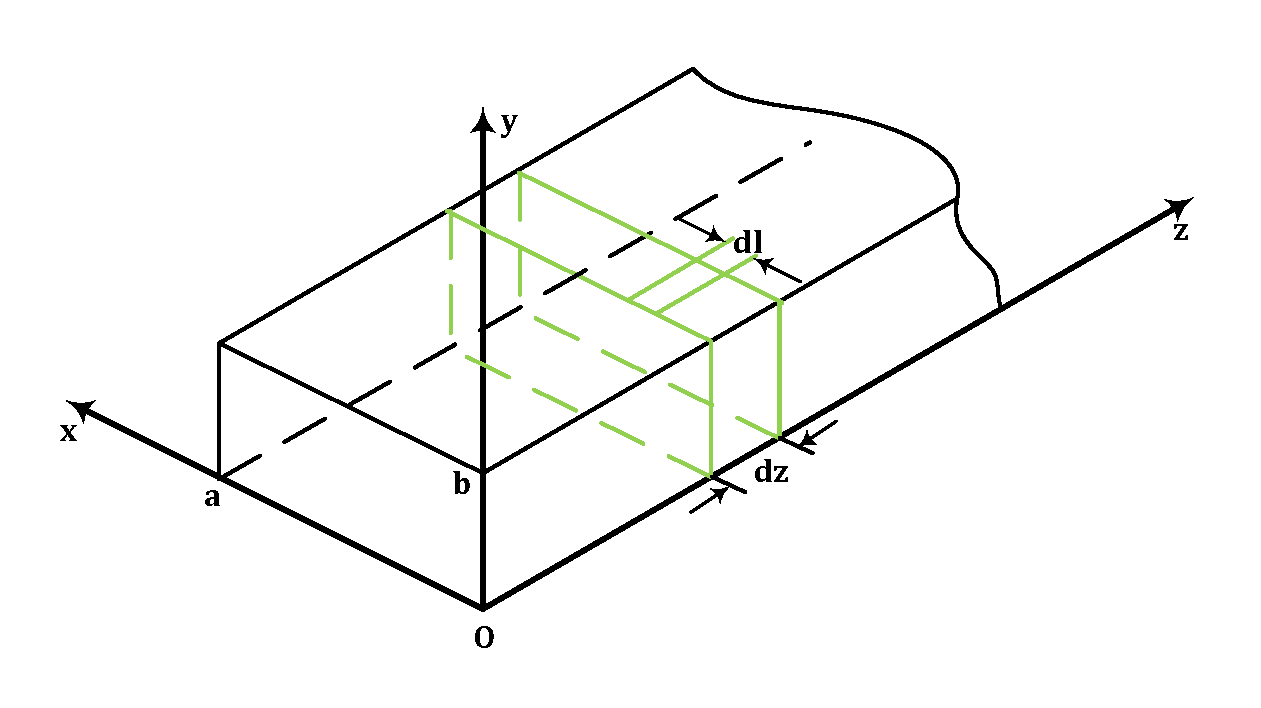
\includegraphics[width=10cm]{Cha6//fig6-9.pdf}
        \caption{衰减计算用图}
        \label{fig6-9}
    \end{figure}
\end{frame}

\begin{frame}{矩形波导——传输特性}
    一般认为波导内媒质是无耗的,所谓衰减是指电流的壁损耗。如图\ref{fig6-9}所示,假定$P_0$是理想导体波导的传输功率,则
    \begin{gather*}
        P=P_0\mathrm{e}^{-2\alpha z}\\
        \frac{\mathrm{d}P}{\mathrm{d}z}=-2\alpha P_0\mathrm{e}^{-2\alpha z}\\
        \alpha=\frac{\mathrm{d}P/\mathrm{d}z}{-2P}=\frac{P_L}{2P}
    \end{gather*}
    $P_L=-\frac{\mathrm{d}P}{\mathrm{d}z}$表示单位长度的功率损耗,负号代表功率减少。在小衰减的条件下,$P\approx P_0$于是
    $$\alpha\approx\frac{P_L}{2P_0}$$
    在波导内壁$\mathrm{d}\sigma=\mathrm{d}l\mathrm{d}z$上衰减功率
    $$\delta P_L=\frac{1}{2}J_{sm}^2R_s\mathrm{d}l\mathrm{d}z$$
    式中,$J_{sm}$为表面电流密度;$R_s$为表面电阻
\end{frame}

\begin{frame}{矩形波导——传输特性}
    \begin{align*}
        \oint_C\delta P_L=\frac{1}{2}\oint_CJ_{sm}^2 & R_s\mathrm{d}l\mathrm{d}z=\frac{1}{2}R_s\mathrm{d}z\oint_CJ_{sm}^2\mathrm{d}l=\frac{1}{2}R_s\mathrm{d}z\oint_C H_{sm}^2\mathrm{d}l \\
                                                     & P_L=-\frac{\mathrm{d}P}{\mathrm{d}z}=\frac{1}{2}R_s\oint_C H_{sm}^2\mathrm{d}l
    \end{align*}
    \begin{align*}
        P_0=\frac{1}{2}\iint_S E_{tm}H_{tm}\mathrm{d}S=\frac{1}{2}\eta\iint_S H^2_{tm}\mathrm{d}S
    \end{align*}
    \begin{empheq}[box=\fbox]{align*}
        &\alpha=\frac{P_L}{2P_0}=\frac{R_s}{2\eta}\frac{\oint_C H_{sm}^2\mathrm{d}l}{\iint_S H_{tm}^2\mathrm{d}S}\quad\mathrm{NP/m}\\
        &\eta=\frac{\sqrt{\frac{\mu}{\epsilon}}}{\sqrt{1-\left(\frac{\lambda}{2a}\right)^2}},R_s=\sqrt{\frac{\omega\mu}{2\sigma}}
    \end{empheq}
\end{frame}

\begin{frame}{矩形波导——传输特性}
    矩形波导$TE_{10}$模的衰减
    \begin{align*}
        \oint_C H_{sm}^2\mathrm{d}l & =2\int_0^a(H_x^2+H_z^2)|_{y=0}\mathrm{d}x+2\int_0^b(H_x^2+H_z^2)|_{x=0}\mathrm{d}y \\
                                    & =aH_0^2\left[\left(\frac{\beta a}{\pi}\right)^2+1\right]+2bH_0^2
    \end{align*}
    \begin{align*}
        \iint_S H_{tm}^2\mathrm{d}S=\int_0^a\int_0^b H_x^2\mathrm{d}x\mathrm{d}y=\frac{ab}{2}\left(\frac{\beta a}{\pi}\right)^2H_0^2
    \end{align*}
    \begin{align*}
        \alpha = \frac{P_L}{2P_0}=\frac{R_s}{2\eta}\frac{\oint_C H_{sm}^2\mathrm{d}l}{\iint_S H_{tm}^2\mathrm{d}S} =
        \frac{R_s}{b\sqrt{\frac{\mu}{\epsilon}}\sqrt{1-\left(\frac{\lambda}{2a}\right)^2}}\left[1+\frac{2b}{a}\left(\frac{\lambda}{2a}\right)^2\right]
    \end{align*}
\end{frame}

\begin{frame}{矩形波导——本征模}
    以矩形波导为例,尽管在z方向它们只可能是入射波加反射波,但是由于横向边界条件,它们由$TE_{mn}$和$TM_{mn}$模组成并且它们只能由
    组成(后者称为完备性),矩形波导中这些模的全部波的完备集合——即本征模。\\
    \hspace*{\fill}\\
    任何情况的可能解,只能在本征模里找,具体场合所不同的仅仅是比例和组合系数,事实上,这样就把求复杂场\uline{函数}的问题变换成求各个模式的\uline{系数}。
\end{frame}

\begin{frame}{矩形波导——本征模}
    \begin{itemize}
        \item 完备性\\
              矩形波导中不论放置什么障碍物和边界条件,它们里边存在的是$TE_{mn}$和$TM_{mn}$模式,而且,它们也只能存在$TE_{mn}$和$TM_{mn}$模式,具体情况
              所不同的仅仅是各种模式的比例和组合。
        \item 正交性\\
              本征模中各个模式是相互正交的,也就是说,它们之间没有功率和能量的交换,即各模式相互独立,在$Fourier$分析中表明
              \begin{align*}
                  \begin{cases}
                      \int_0^a\sin\left(\frac{m\pi}{a}x\right)\left\{\begin{aligned}\cos \\ \sin\end{aligned}\left(\frac{l\pi}{a}x\right)\right\}\mathrm{d}x=0 \quad m\neq l \\
                      \int_0^b\sin\left(\frac{n\pi}{b}x\right)\left\{\begin{aligned}\cos \\ \sin\end{aligned}\left(\frac{p\pi}{b}y\right)\right\}\mathrm{d}y=0 \quad n\neq p
                  \end{cases}
              \end{align*}
              上式保证了每一种模式的独立性
    \end{itemize}
\end{frame}

\begin{frame}{矩形波导——本征模}
    \begin{itemize}
        \item 传输模和消失模(evanescent mode)\\
              由于频率的选择,每一种模都有可能成为传输模或消失模\\
              截止波数:
              $$k_c=\sqrt{k_x^2+k_y^2}=\sqrt{\left(\frac{m\pi}{a}\right)^2+\left(\frac{n\pi}{b}\right)^2}=\frac{2\pi}{\lambda_{cmn}}$$
              \begin{enumerate}
                  \item 传输模 \quad $\lambda<\lambda_{cmn}$\\
                        \begin{columns}
                            \begin{column}{0.5\linewidth}
                                \begin{gather*}
                                    \mathrm{e}^{-\mathrm{j}\beta z}\\
                                    \beta=(2\pi/\lambda)\sqrt{1-(\lambda/\lambda_c)^2}
                                \end{gather*}
                            \end{column}
                            \begin{column}{0.5\linewidth}
                                \begin{figure}
                                    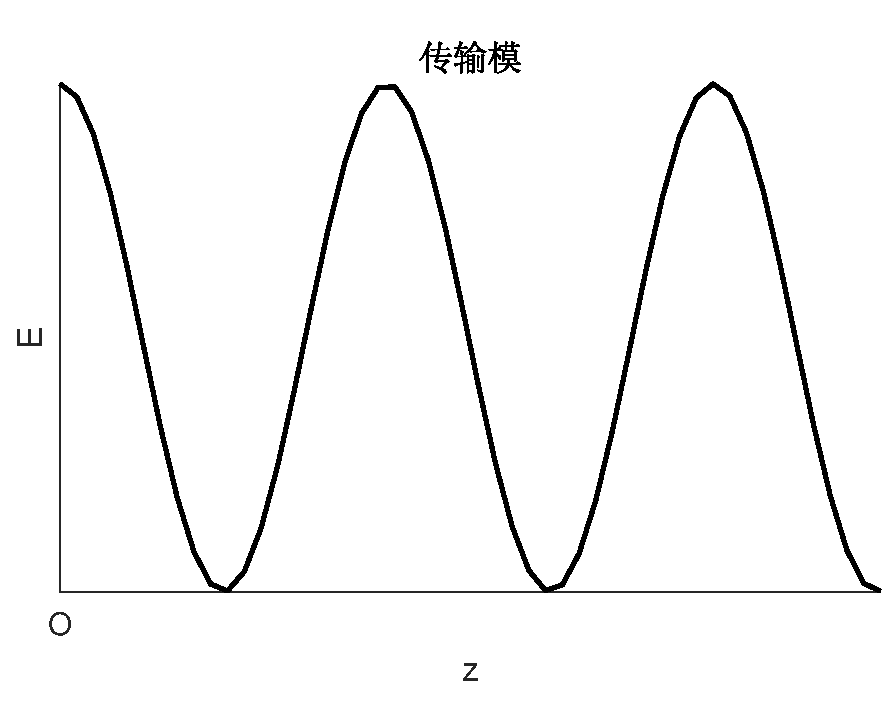
\includegraphics[width=5cm]{Cha6//fig6-10.pdf}
                                \end{figure}
                            \end{column}
                        \end{columns}
                        \saveenum
              \end{enumerate}
    \end{itemize}
\end{frame}

\begin{frame}{矩形波导——本征模}
    \begin{itemize}
        \item 传输模和消失模(evanescent mode)\\
              \begin{enumerate}
                  \resume
                  \item 消失模 \quad $\lambda>\lambda_{cmn}$\\
                        \begin{columns}
                            \begin{column}{0.5\linewidth}
                                \begin{gather*}
                                    \mathrm{e}^{-\gamma z}\\
                                    \gamma=(2\pi/\lambda_c)\sqrt{1-(\lambda_c/\lambda)^2}
                                \end{gather*}
                            \end{column}
                            \begin{column}{0.5\linewidth}
                                \begin{figure}
                                    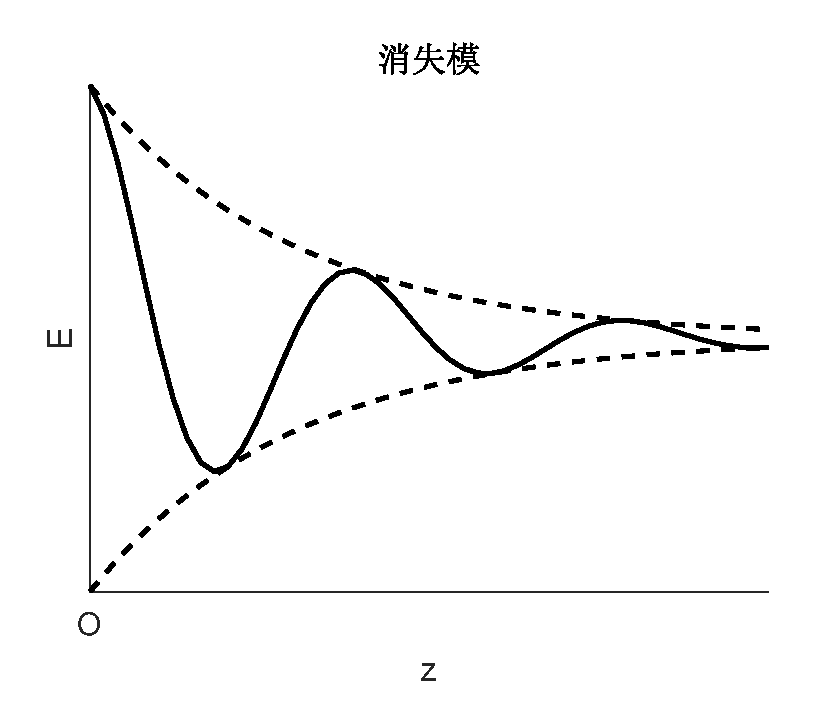
\includegraphics[width=5cm]{Cha6//fig6-11.pdf}
                                \end{figure}
                            \end{column}
                        \end{columns}
              \end{enumerate}
    \end{itemize}
\end{frame}

\begin{frame}{矩形波导}
    主模$TE_{10}$模小结
    \begin{align*}
        \begin{cases}
            E_y=\frac{-\mathrm{j}\omega\mu a}{\pi}H_{10}\sin\frac{\pi x}{a}\mathrm{e}^{-\mathrm{j}\beta z} \\
            H_x=\frac{\mathrm{j}\beta a}{\pi}H_{10}\sin\frac{\pi x}{a}\mathrm{e}^{-\mathrm{j}\beta z}      \\
            H_z=H_{10}\cos\frac{\pi x}{a}\mathrm{e}^{-\mathrm{j}\beta z}                                   \\
            E_x=E_z=H_y=0                                                                                  \\
        \end{cases}
    \end{align*}

    \begin{figure}
        \flushright
        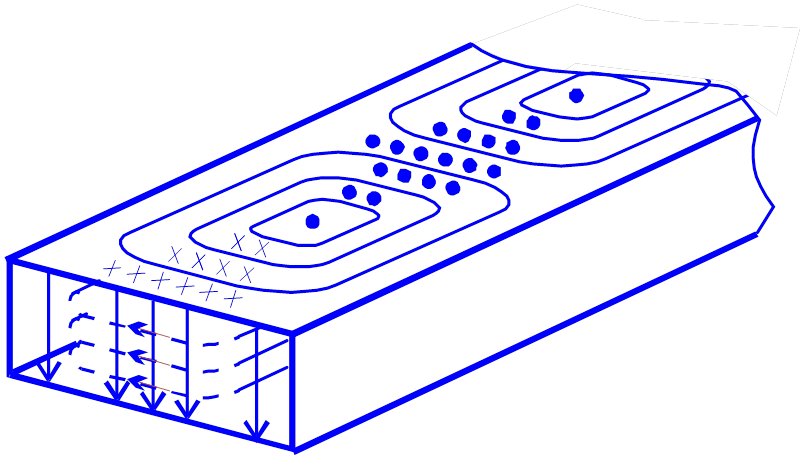
\includegraphics[width=6cm]{Cha6//fig6-12.png}
    \end{figure}
\end{frame}

\begin{frame}{矩形波导}
    \begin{columns}
        \begin{column}{0.5\linewidth}
            \begin{itemize}
                \item 传播条件:\\
                      $\lambda<\lambda_c=2a$
                \item 波导波长:\\
                      $\lambda_g=\dfrac{\lambda}{\sqrt{1-(\lambda/2a)^2}}$
                \item 相速:\\
                      $v_p=\dfrac{C}{\sqrt{1-(\lambda/2a)^2}}$
                \item 波阻抗:\\
                      $\eta=\sqrt{\dfrac{\mu}{\epsilon}}\dfrac{1}{\sqrt{1-(\lambda/2a)^2}}$
            \end{itemize}
        \end{column}
        \begin{column}{0.5\linewidth}
            \begin{figure}
                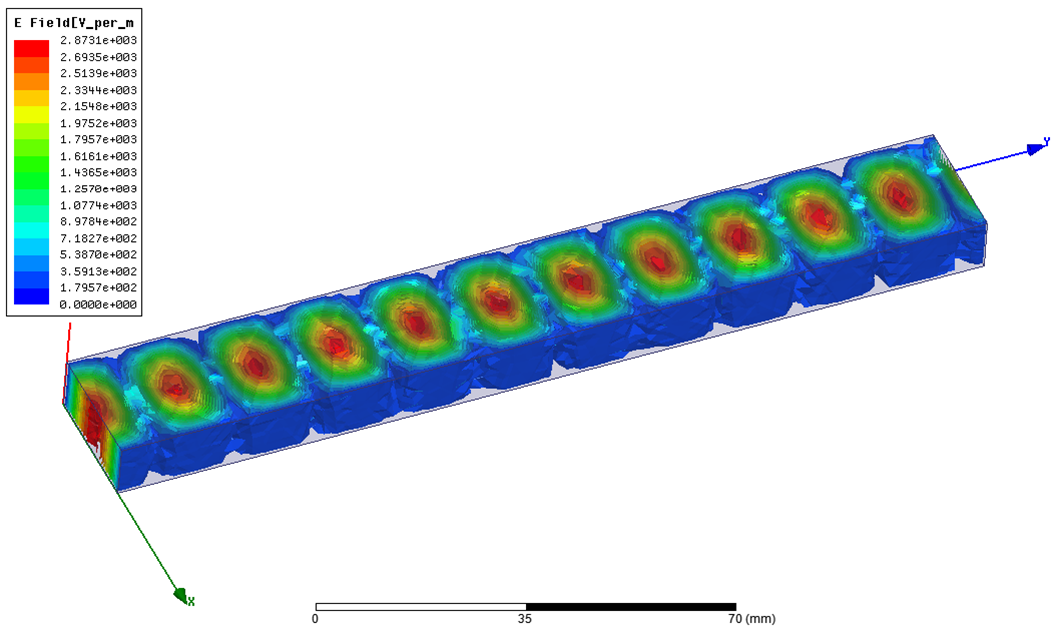
\includegraphics[width=5.5cm]{Cha6//fig6-13.png}
                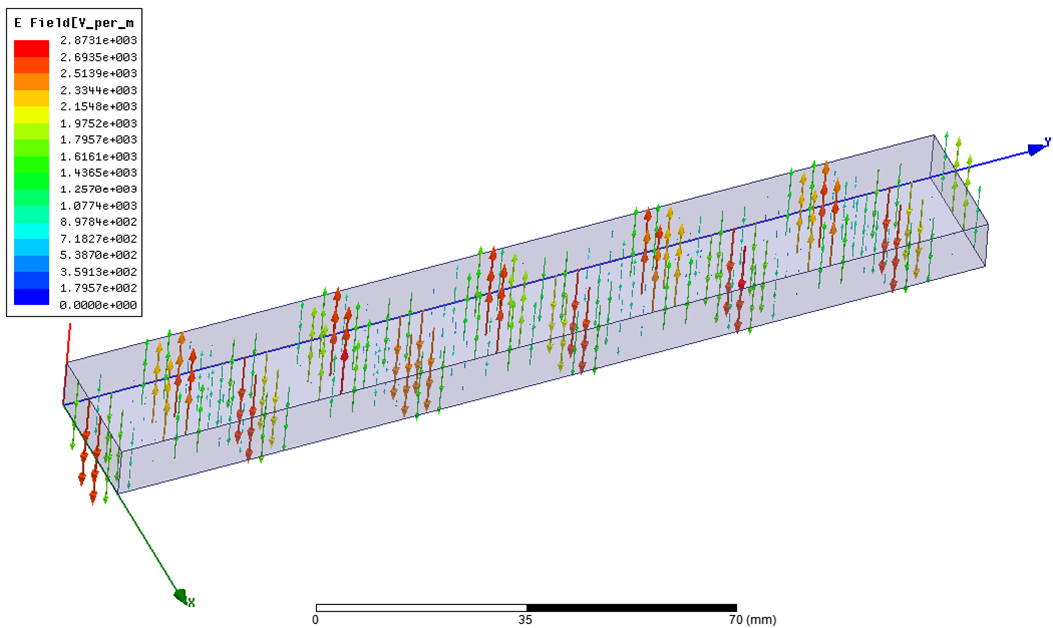
\includegraphics[width=5.5cm]{Cha6//fig6-14.png}
            \end{figure}
        \end{column}
    \end{columns}

\end{frame}

\begin{frame}{矩形波导}
    $TE_{10}$波表达式,是以$H_z$为领矢矢量,然而在实用上,也可以用$E_y$作为领矢矢量
    \begin{gather*}
        E_y=E_0\sin\left(\frac{\pi}{a}x\right)\mathrm{e}^{-\mathrm{j}\beta z}\\
        \nabla\times\vec{E}=-\mathrm{j}\omega\mu\vec{H}\\
        \begin{bmatrix*}
            \hat{i} & \hat{j} & \hat{k}\\
            \frac{\partial}{\partial x} & \frac{\partial}{\partial y} & -\mathrm{j}\beta\\
            0 & E_y & 0
        \end{bmatrix*}
        =\mathrm{j}\beta E_y\hat{i}+\frac{\partial E_y}{\partial x}\hat{k}=-\mathrm{j}\omega\mu(H_x\hat{i}+H_y\hat{j}+H_z\hat{k})\\
        E_y = E_0\sin\left(\frac{\pi}{a}x\right)\mathrm{e}^{-\mathrm{j}\beta z}\\
        H_x = -\frac{\beta}{\omega\mu}E_0\sin\left(\frac{\pi}{a}x\right)\mathrm{e}^{-\mathrm{j}\beta z}\\
        H_z = \mathrm{j}\frac{1}{\omega\mu}\left(\frac{\pi}{a}\right)E_0\cos\left(\frac{\pi}{a}x\right)\mathrm{e}^{-\mathrm{j}\beta z}
    \end{gather*}
\end{frame}

\begin{frame}{矩形波导}
    [例1] BJ-100波导,$a\times b=22.86\times 10.16 mm^2$,求单模传输的波长范围和频率范围。\\
    \hspace*{\fill}
    \flushleft
    [解] 已经知道单模传输条件是 \quad $\lambda_{cmn}<\lambda<2a$ \\
    \begin{align*}
         & \lambda_{c10}=2a=45.72mm \quad \lambda_{c11}=\frac{2}{\sqrt{(1/a)^2+(1/b)^2}}=18mm    \\
         & \lambda_{c20}=a=22.86mm \quad  \lambda_{c21}=\frac{2}{\sqrt{(2/a)^2+(1/b)^2}}=15.10mm \\
         & \lambda_{c01}=2b=20.32mm \quad \lambda_{c30}=\frac{2}{3}a=15.25mm
    \end{align*}
\end{frame}

\begin{frame}{矩形波导}
    十分明显,第二模式是$\lambda_{c20}=22.86mm$。因此,单模传输
    \begin{align*}
        22.86mm< & \lambda<45.72mm \\
                 & \downarrow      \\
        6.55GHz< & f<13.10GHz
    \end{align*}
    \begin{figure}
        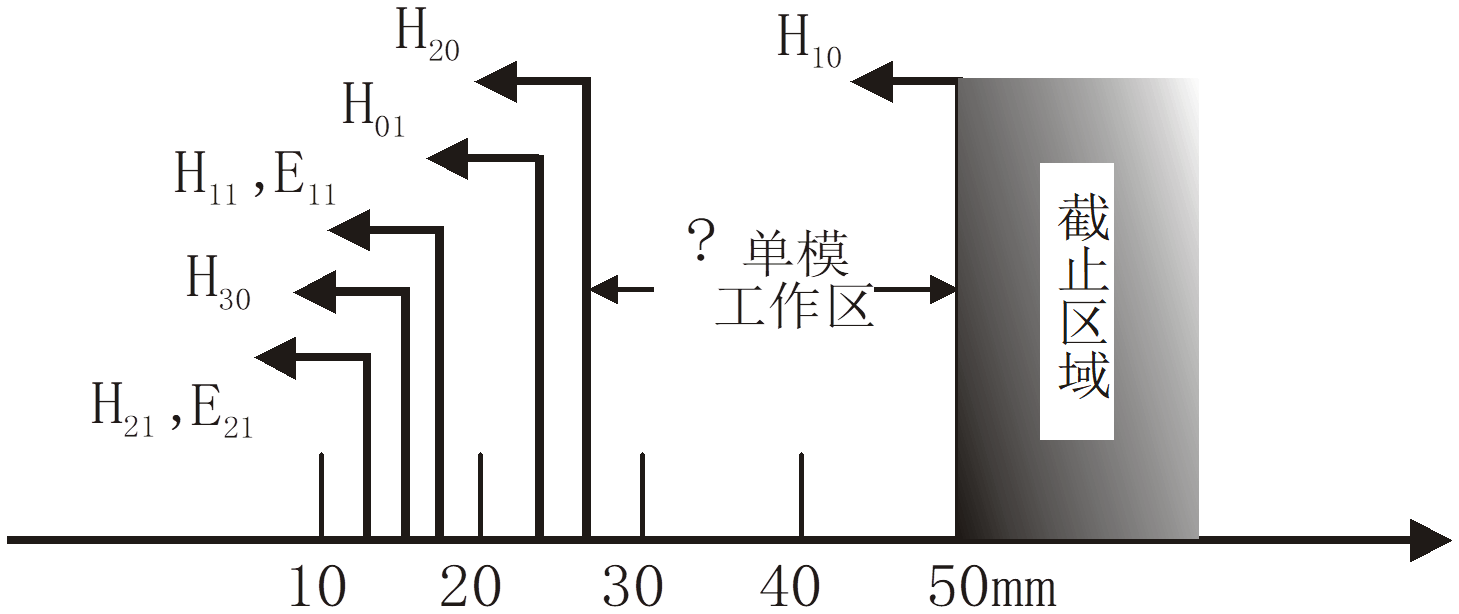
\includegraphics[width=8cm]{Cha6//fig6-15.png}
    \end{figure}
\end{frame}

\subsection{圆波导}
\begin{frame}{圆波导}
    圆波导是横截面为圆形的空心金属管,如图所示,其尺寸半径为$R$。
    \begin{columns}
        \begin{column}{0.4\linewidth}
            \begin{enumerate}
                \item 圆波导的提出来自实践的需要。例如,雷达的旋转搜索,如果没有旋转关节,那只好发射机跟着转。像这类应用中,圆波导成为必须器件。
                      \saveenum
            \end{enumerate}
        \end{column}
        \begin{column}{0.6\linewidth}
            \begin{figure}
                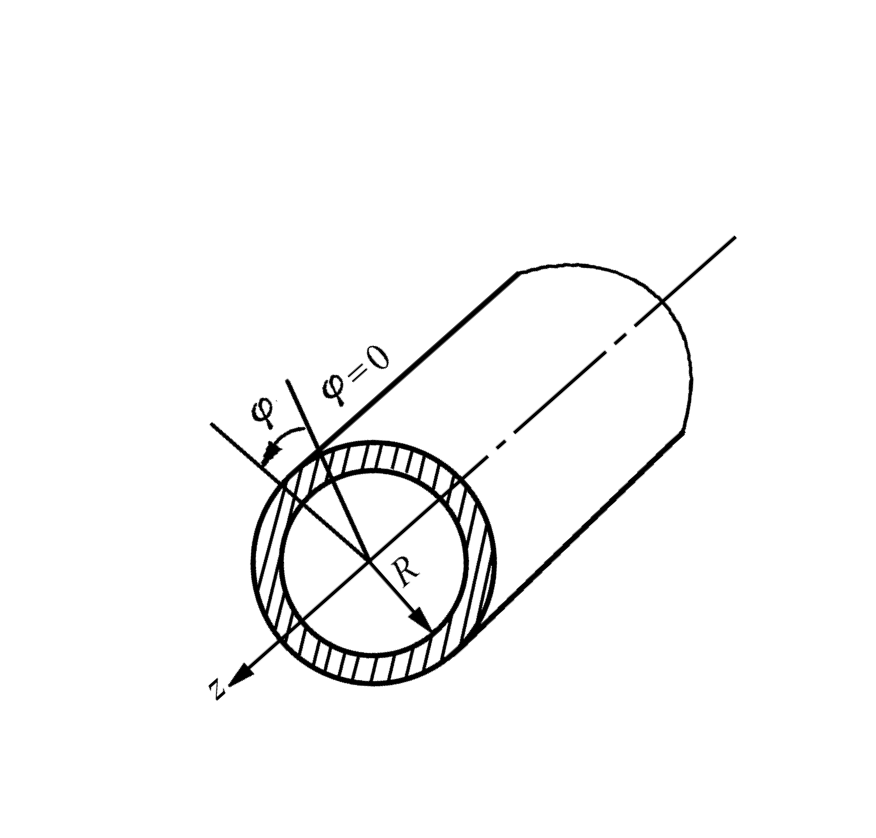
\includegraphics[width=6cm]{Cha6//fig6-16.png}
            \end{figure}
        \end{column}
    \end{columns}
    以后要用到的极化衰减器,多模或波纹喇叭,都会应用到圆波导。可以这样说,几何对称性给圆波导带来广泛的用途和价值。
\end{frame}

\begin{frame}{圆波导}
    \begin{enumerate}
        \resume
        \item 从力学和应力平衡角度,机加工圆波导更为有利,对于误差和方便性等方面均略胜矩形波导一筹
        \item 根据微波传输线的研究发现:功率容量和衰减是十分重要的两个指标。这个问题从广义上看\\
              \begin{align*}
                  \begin{cases}
                      \textbf{功率容量}\quad P_{max}\propto S (S是截面) \\
                      \textbf{衰减} \quad \alpha \propto L (L是周长)
                  \end{cases}
              \end{align*}
              引出一个品质因数$F$
              $$F=\frac{P_{max}}{\alpha}=\frac{S}{L}$$
              很明显,在相同周长条件下,圆面积最大
              \saveenum
    \end{enumerate}
\end{frame}

\begin{frame}{圆波导}
    \begin{enumerate}
        \resume
        \item 矩形波导中存在的一个矛盾\\
              当我们深入研究波导衰减,发现频率升高时,衰减在矩形波导中上升很快。仔细分析表明,衰减由两部分组成:一部分成为纵向电流衰减,另一部分是横向电流衰减。\\
              当频率升高时,横向电尺寸加大,使横向电流衰减反而减少。这样所构成的矛盾因素使衰减有了极值。\\
              而以后在圆波导中将会发现,有的波型无纵向电流,因此,若采用这种波形会使高频时衰减减小。
    \end{enumerate}
    \begin{figure}
        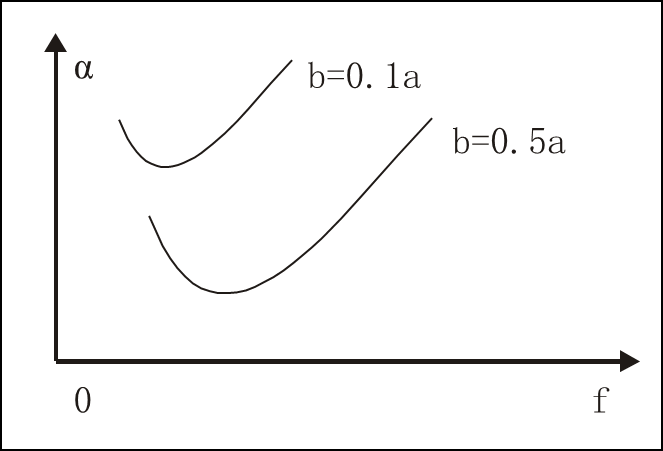
\includegraphics[width=5cm]{Cha6//fig6-17.png}
    \end{figure}
\end{frame}

\begin{frame}{圆波导}
    由于圆波导具有\textcolor{blue}{损耗较小}和\textcolor{blue}{双极化}特性,所以常用作天线馈线和微波谐振腔,也可用作较远距离的传输线。\\
    \hspace*{\fill}\\
    根据圆波导具有的轴对称性,宜采用圆柱坐标系来分析。
\end{frame}

\begin{frame}{圆波导——导模}
    \begin{itemize}
        \item 圆形波导一般解\\
              在圆柱坐标下\\
              $$\nabla^2=\frac{1}{r}\frac{\partial}{\partial r}\left(r\frac{\partial}{\partial r}\right)+\frac{1}{r^2}\frac{\partial^2}{\partial\varphi^2}+\frac{\partial^2}{\partial z^2}$$
              纵向场分量满足Helmholtz方程
              \begin{align*}
                  \left(\frac{\partial^2}{\partial r^2}+\frac{1}{r}\frac{\partial}{\partial r}+\frac{1}{r^2}\frac{\partial^2}{\partial\varphi^2}+k_c^2\right)\left\{\begin{matrix*}E_z(r,\varphi)\\H_z(r,\varphi)\end{matrix*}\right\}=0
              \end{align*}
    \end{itemize}
    \begin{figure}
        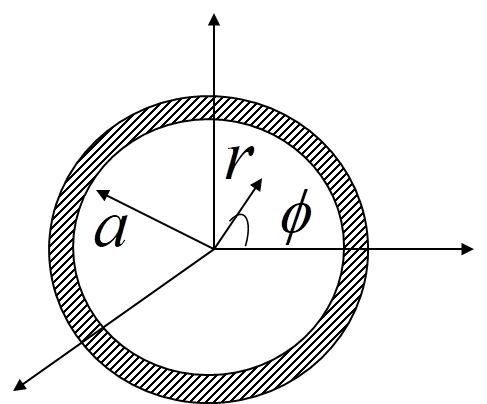
\includegraphics[width=4cm]{Cha6//fig6-18.png}
    \end{figure}
\end{frame}

\begin{frame}{圆波导——导模}
    以TE波为例,即$E_z=0$
    \begin{gather*}
        H_z=R(r)\Phi(\varphi)Z(z)\\
        Z(z)=c\mathrm{e}^{-\mathrm{j}\beta z}\rightarrow H_z=R(r)\Phi(\varphi)\mathrm{e}^{-\mathrm{j}\beta z}
    \end{gather*}
    代入到Helmholtz方程有:
    \begin{gather*}
        \frac{\partial^2H_z}{\partial r^2}+\frac{1}{r}\frac{\partial H_z}{\partial r}+\frac{1}{r^2}\frac{\partial^2H_z}{\partial\varphi^2}=-k_c^2H_z\quad k_c^2=k^2-\beta^2\\
        \begin{cases}
            \dfrac{1}{\Phi}\dfrac{\mathrm{d}^2\Phi}{\mathrm{d}\varphi^2}=-m^2 \\
            r^2\dfrac{\mathrm{d}^2R}{\mathrm{d}r^2}+r\dfrac{\mathrm{d}R}{\mathrm{d}r}+(k_c^2r^2-m^2)R=0
        \end{cases}
    \end{gather*}
\end{frame}

\begin{frame}{圆波导——导模}
    其解分别是
    \begin{align*}
        \begin{cases}
            \Phi(\varphi)=c_1\cos m\varphi+c_2\sin m\varphi=\left\{\begin{matrix*}\cos m\varphi \\ \sin m\varphi\end{matrix*}\right\} \\
            R(r)=c_3J_m(k_c r)+c_4Y_m(k_c r)=\left\{\begin{matrix*}J_m(k_c r)\\Y_m(k_c r)\end{matrix*}\right\}
        \end{cases}
    \end{align*}
    其中$c_1,c_2,c_3,c_4$为常数。$m=0,1,2,\cdots$为整数。\\
    边界条件:\\
    \begin{enumerate}
        \item 有限条件:$R(r=0)$有限性
        \item 周期性:$\Phi(\varphi=0)=\Phi(\varphi=2\pi)$
        \item 理想导体条件:切向分量为零
    \end{enumerate}
    本征解
    $$H_z=H_0J_m(k_cr)
        \begin{matrix}
            \cos m\varphi \\
            \sin m\varphi
        \end{matrix}
        \mathrm{e}^{-\mathrm{j}\beta z}$$
\end{frame}

\begin{frame}{圆波导——导模}
    \begin{columns}
        \begin{column}{0.5\linewidth}
            \begin{figure}
                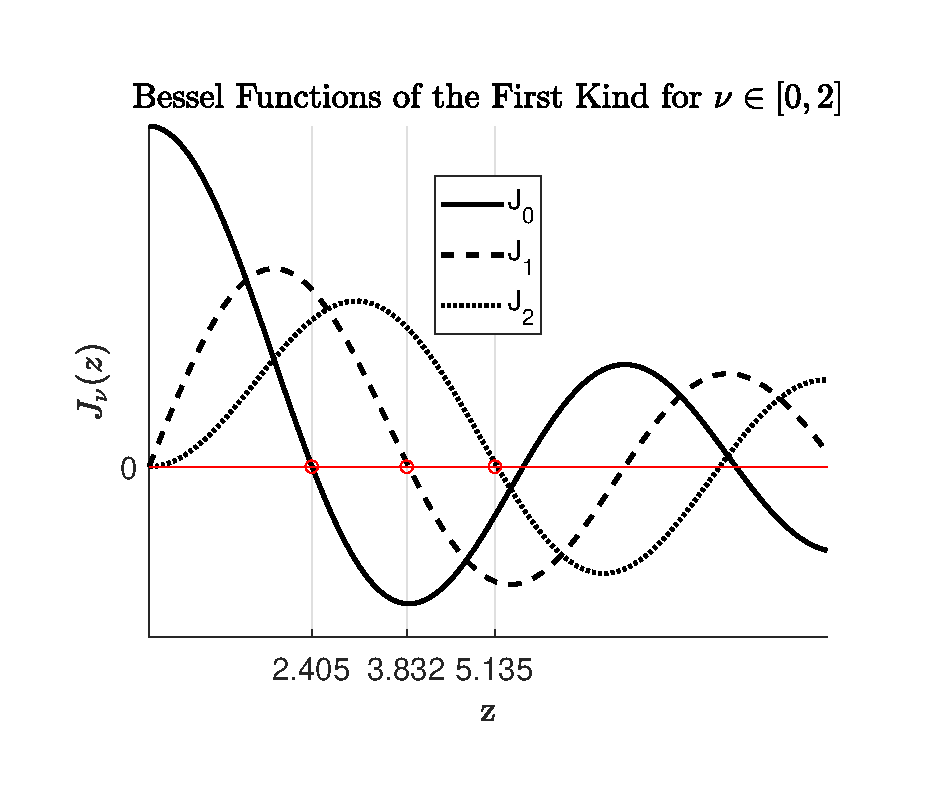
\includegraphics[width=6cm]{Cha6//fig6-19.pdf}
            \end{figure}
        \end{column}
        \begin{column}{0.5\linewidth}
            \begin{figure}
                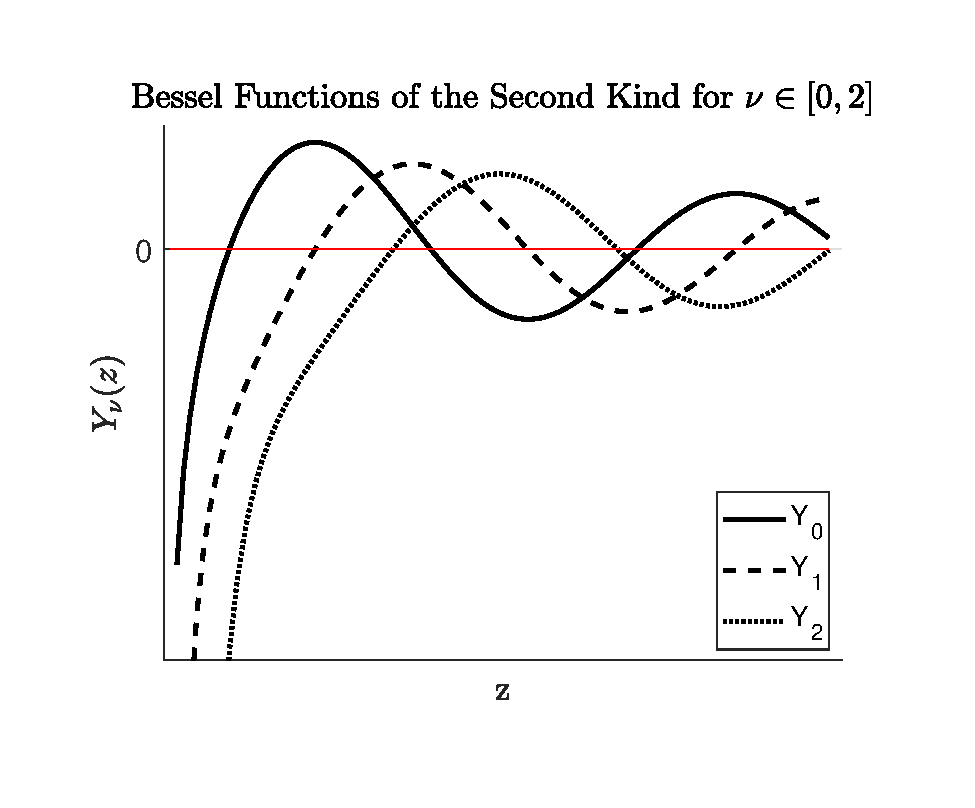
\includegraphics[width=6cm]{Cha6//fig6-19-2.pdf}
            \end{figure}
        \end{column}
    \end{columns}
\end{frame}

\begin{frame}{圆波导——导模}
    \begin{itemize}
        \item 纵向分量法\\
              利用纵向分量法表示横向分量\\
              \begin{gather*}
                  \nabla\times\vec{H}=\mathrm{j}\omega\epsilon\vec{E}\qquad
                  \begin{cases}
                      \dfrac{1}{r}\dfrac{\partial H_z}{\partial\varphi}-\dfrac{\partial H_{\varphi}}{\partial z}=\mathrm{j}\omega\epsilon E_r \\
                      \dfrac{\partial H_r}{\partial z}-\dfrac{\partial H_z}{\partial r}=\mathrm{j}\omega\epsilon E_{\varphi}                  \\
                      \dfrac{1}{r}\left[\dfrac{\partial}{\partial r}(rH_{\varphi})-\dfrac{\partial H_r}{\partial\varphi}\right]=\mathrm{j}\omega\epsilon E_z
                  \end{cases}\\
                  \nabla\times\vec{E}=-\mathrm{j}\omega\mu\vec{H}\qquad
                  \begin{cases}
                      \dfrac{1}{r}\dfrac{\partial E_z}{\partial\varphi}-\dfrac{\partial E_{\varphi}}{\partial z}=-\mathrm{j}\omega\mu H_r \\
                      \dfrac{\partial E_r}{\partial z}-\dfrac{\partial E_z}{\partial r}=-\mathrm{j}\omega\mu H_{\varphi}                  \\
                      \dfrac{1}{r}\left[\dfrac{\partial}{\partial r}(rE_{\varphi})-\dfrac{\partial E_r}{\partial\varphi}\right]=-\mathrm{j}\omega\mu H_z
                  \end{cases}
              \end{gather*}
    \end{itemize}
\end{frame}

\begin{frame}{圆波导——导模}
    \begin{gather*}
        \begin{bmatrix*}
            E_r\\
            H_{\varphi}\\
            H_r\\
            E_{\varphi}\\
        \end{bmatrix*}
        =\dfrac{1}{k_c^2}
        \begin{bmatrix*}
            -\gamma & 0 & 0 & -\mathrm{j}\omega\mu \\
            0 & -\gamma & \mathrm{j}\omega\mu & 0 \\
            0 & \mathrm{j}\omega\epsilon & -\gamma & 0 \\
            -\mathrm{j}\omega\epsilon & 0 & 0 & -\gamma \\
        \end{bmatrix*}
        \begin{bmatrix*}
            \dfrac{\partial E_z}{\partial r} \\
            \dfrac{1}{r}\dfrac{\partial E_z}{\partial\varphi}\\
            \dfrac{\partial H_z}{\partial r}\\
            \dfrac{1}{r}\dfrac{\partial H_z}{\partial\varphi}\\
        \end{bmatrix*}
    \end{gather*}
    边界条件
    \begin{gather*}
        \begin{matrix*}
            E_{0\varphi}(r,\varphi)|_{r=a}=0 & TE导波 \\
            E_{0z}(r,\varphi)|_{r=a}=0 & TM导波 \\
        \end{matrix*}
    \end{gather*}
\end{frame}

\begin{frame}{圆波导——TE模}
    \begin{gather*}
        H_z(r,\varphi,z)=H_0J_m(k_cr)
        \begin{matrix*}
            \cos m\varphi \\
            \sin m\varphi \\
        \end{matrix*}
        \mathrm{e}^{-\mathrm{j}\beta z}\\
        E_{\varphi}(r,\varphi,z)=\frac{\mathrm{j}\omega\mu}{k_c}H_0J_m^{'}(k_cr)
        \begin{matrix*}
            \cos m\varphi \\
            \sin m\varphi \\
        \end{matrix*}
        \mathrm{e}^{-\mathrm{j}\beta z}\\
        E_{0\varphi}(r,\varphi)|_{r=a}=0 \quad J_m^{'}(k_c a)=0
    \end{gather*}
    令$u_{mn}^{'}$为Bessel函数导数的根,本征值
    $$k_{cmn}=u_{mn}^{'}/a \quad n=1,2,\cdots$$
\end{frame}

\begin{frame}{圆波导——TE模}
    \begin{table}
        \begin{threeparttable}[b]
            \caption{圆波导中$TE$模截止波长值}
            \setlength{\tabcolsep}{9mm}{ %调整表格宽度,效果为“按页面宽度调整表格”
                \begin{tabular}{ccc}
                    \toprule
                    波型       & $u_{mn}^{'}$ & $\lambda_c$\tnote{1} \\ \hline
                    $H_{11}$ & 1.841        & 3.41$a$              \\
                    $H_{21}$ & 3.054        & 2.06$a$              \\
                    $H_{01}$ & 3.832        & 1.64$a$              \\
                    \bottomrule
                \end{tabular}
            }
            \begin{tablenotes}
                \item[1] \footnotesize{$\lambda_{cmn}=\frac{2\pi a}{u_{mn}^{'}}$}
            \end{tablenotes}
        \end{threeparttable}
    \end{table}
\end{frame}

\begin{frame}{圆波导——TE模}
    $TE$基本解为
    \begin{align*}
        \begin{cases}
            E_z=0                                     \\
            H_z(r,\varphi,z)=\sum\limits_{m=0}^{\infty}\sum\limits_{n=1}^{\infty}H_{mn}J_m\left(\dfrac{u_{mn}^{'}}{a}r\right)
            \begin{matrix*}
                \cos m\varphi\\
                \sin m\varphi\\
            \end{matrix*}
            \mathrm{e}^{\mathrm{j}(\omega t-\beta z)} \\
            E_r=\pm\sum\limits_{m=0}^{\infty}\sum\limits_{n=1}^{\infty}\dfrac{\mathrm{j}\omega\mu ma^2}{(u_{mn}^{'})^2r}H_{mn}J_m\left(\dfrac{u_{mn}^{'}}{a}r\right)
            \begin{matrix*}
                \sin m\varphi\\
                \cos m\varphi\\
            \end{matrix*}
            \mathrm{e}^{\mathrm{j}(\omega t-\beta z)} \\
            E_{\varphi}=\sum\limits_{m=0}^{\infty}\sum\limits_{n=1}^{\infty}\dfrac{\mathrm{j}\omega\mu a}{u_{mn}^{'}}H_{mn}J_m^{'}\left(\dfrac{u_{mn}^{'}}{a}r\right)
            \begin{matrix*}
                \cos m\varphi\\
                \sin m\varphi\\
            \end{matrix*}
            \mathrm{e}^{\mathrm{j}(\omega t-\beta z)} \\
            H_r=\sum\limits_{m=0}^{\infty}\sum\limits_{n=1}^{\infty}-\dfrac{\mathrm{j}\beta a}{u_{mn}^{'}}H_{mn}J_m^{'}\left(\dfrac{u_{mn}^{'}}{a}r\right)
            \begin{matrix*}
                \cos m\varphi\\
                \sin m\varphi\\
            \end{matrix*}
            \mathrm{e}^{\mathrm{j}(\omega t-\beta z)} \\
            H_{\varphi}=\pm\sum\limits_{m=0}^{\infty}\sum\limits_{n=1}^{\infty}\dfrac{\mathrm{j}\beta ma^2}{(u_{mn}^{'})^2r}H_{mn}J_m\left(\dfrac{u_{mn}^{'}}{a}r\right)
            \begin{matrix*}
                \sin m\varphi\\
                \cos m\varphi\\
            \end{matrix*}
            \mathrm{e}^{\mathrm{j}(\omega t-\beta z)} \\
        \end{cases}
    \end{align*}
\end{frame}

\begin{frame}{圆波导——TE模}
    波型指数$n$表示场沿半径分布的最大值个数\\
    \hspace*{\fill}\\
    圆波导$TE$模的波阻抗为
    $$Z_{TE}=\frac{E_r}{H_{\varphi}}=-\frac{E_{\varphi}}{H_r}=\frac{\omega\mu}{\beta}=\frac{k\eta}{\beta}$$
    传播常数
    $$\beta_{mn}=\sqrt{k^2-k_{cmn}^2}=\sqrt{k^2-(u_{mn}^{'}/a)^2}$$
    截止波长
    $$\lambda_{cmn}=2\pi a/u_{mn}^{'}$$
    截止频率
    $$f_{cmn}=\frac{k_{cmn}}{2\pi\sqrt{\mu\epsilon}}=\frac{u_{mn}^{'}}{2\pi a\sqrt{\mu\epsilon}}$$
\end{frame}

\begin{frame}{圆波导——TM模}
    完全类似,用边界条件确定$k_c$\\
    \hspace*{\fill}\\
    在$r=a$处,$E_{\varphi}=0,E_z=0$,即\\
    \begin{empheq}[box=\fbox]{align*}
        J_m(k_ca)=0
    \end{empheq}
    设第一类$Bessel$函数$m$阶第$n$个根为$u_{mn}$,则
    $$k_ca=u_{mn}\qquad n=1,2,\cdots$$
    可得
    $$k_c=\frac{u_{mn}}{a}\qquad \lambda_c=\frac{2\pi a}{u_{mn}}$$
\end{frame}

\begin{frame}{圆波导——TM模}
    $TM$基本解为
    \begin{align*}
        \begin{cases}
            H_z=0                                     \\
            E_z(r,\varphi,z)=\sum\limits_{m=0}^{\infty}\sum\limits_{n=1}^{\infty}E_{mn}J_m\left(\dfrac{u_{mn}}{a}r\right)
            \begin{matrix*}
                \cos m\varphi\\
                \sin m\varphi\\
            \end{matrix*}
            \mathrm{e}^{\mathrm{j}(\omega t-\beta z)} \\
            E_r=\sum\limits_{m=0}^{\infty}\sum\limits_{n=1}^{\infty}-\dfrac{\mathrm{j}\beta a}{u_{mn}}E_{mn}J_m^{'}\left(\dfrac{u_{mn}}{a}r\right)
            \begin{matrix*}
                \cos m\varphi\\
                \sin m\varphi\\
            \end{matrix*}
            \mathrm{e}^{\mathrm{j}(\omega t-\beta z)} \\
            E_{\varphi}=\pm\sum\limits_{m=0}^{\infty}\sum\limits_{n=1}^{\infty}\dfrac{\mathrm{j}\beta ma^2}{u_{mn}^{2}r}E_{mn}J_m\left(\dfrac{u_{mn}}{a}r\right)
            \begin{matrix*}
                \sin m\varphi\\
                \cos m\varphi\\
            \end{matrix*}
            \mathrm{e}^{\mathrm{j}(\omega t-\beta z)} \\
            H_r=\mp\sum\limits_{m=0}^{\infty}\sum\limits_{n=1}^{\infty}\dfrac{\mathrm{j}\omega\epsilon ma^2}{u_{mn}^{2}r}E_{mn}J_m\left(\dfrac{u_{mn}}{a}r\right)
            \begin{matrix*}
                \sin m\varphi\\
                \cos m\varphi\\
            \end{matrix*}
            \mathrm{e}^{\mathrm{j}(\omega t-\beta z)} \\
            H_{\varphi}=\sum\limits_{m=0}^{\infty}\sum\limits_{n=1}^{\infty}\dfrac{-\mathrm{j}\omega\epsilon a}{u_{mn}}E_{mn}J_m^{'}\left(\dfrac{u_{mn}}{a}r\right)
            \begin{matrix*}
                \cos m\varphi\\
                \sin m\varphi\\
            \end{matrix*}
            \mathrm{e}^{\mathrm{j}(\omega t-\beta z)} \\
        \end{cases}
    \end{align*}
\end{frame}

\begin{frame}{圆波导——TM模}
    \begin{table}
        \centering
        \begin{threeparttable}[b]
            \caption{圆波导中$TM$模截止波长值}
            \setlength{\tabcolsep}{9mm}{ %调整表格宽度,效果为“按页面宽度调整表格”
                \begin{tabular}{ccc}
                    \toprule
                    波型       & $u_{mn}$ & $\lambda_c$\tnote{1} \\ \hline
                    $E_{01}$ & 2.405    & 2.62$a$              \\
                    $E_{11}$ & 3.832    & 1.64$a$              \\
                    $E_{21}$ & 5.135    & 1.22$a$              \\
                    \bottomrule
                \end{tabular}
            }
            \begin{tablenotes}
                \item[1] \footnotesize{$\lambda_{cmn}=\frac{2\pi a}{u_{mn}}$}
            \end{tablenotes}
        \end{threeparttable}
    \end{table}
    \begin{columns}
        \begin{column}{0.4\linewidth}
            圆波导$TM$模的波阻抗为
            $$Z_{TM}=\frac{E_r}{H_{\varphi}}=-\frac{E_{\varphi}}{H_r}=\frac{\beta}{\omega\epsilon}$$
        \end{column}
        \begin{column}{0.6\linewidth}
            \begin{figure}
                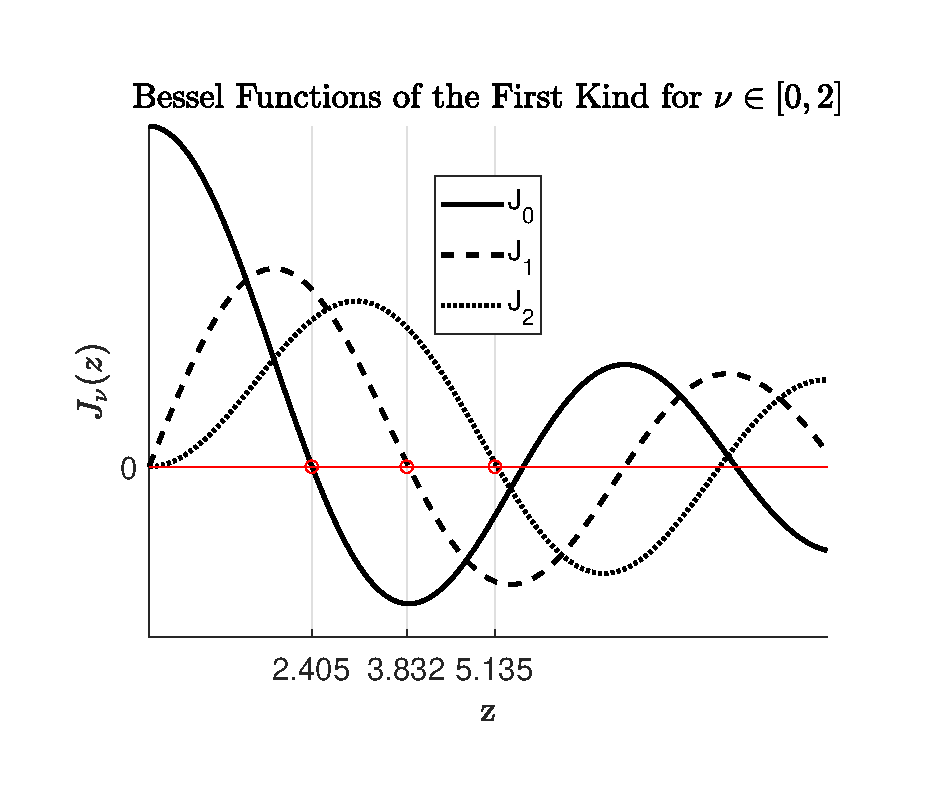
\includegraphics[width=5cm]{Cha6//fig6-19.pdf}
            \end{figure}
        \end{column}
    \end{columns}
\end{frame}

\begin{frame}{圆波导——简并}
    \begin{enumerate}
        \item 圆波导中$TE$模和$TM$模有无限多个\\
              $n=0$表示第$0$个根,也即,$u_{mn}^{'}=u_{mn}\equiv 0$,也即$TE_{m0},TM_{m0}$模不存在。\\
              但是它却可以存在$TE_{0n},TE_{mn},TM_{0n}和TM_{mn}$模,其中$m=0$表示在圆周方向上不变化
        \item $TE$模截止波长取决于$m$阶$Bessel$函数\textbf{导数}第$n$个根\\
              $$\lambda_{cTE}=\frac{2\pi a}{u_{mn}^{'}}$$
              $TM$模截止波长取决于$m$阶$Bessel$函数第$n$个根\\
              $$\lambda_{cTM}=\frac{2\pi a}{u_{mn}}$$
              \saveenum
    \end{enumerate}
\end{frame}

\begin{frame}{圆波导——简并}
    \begin{figure}
        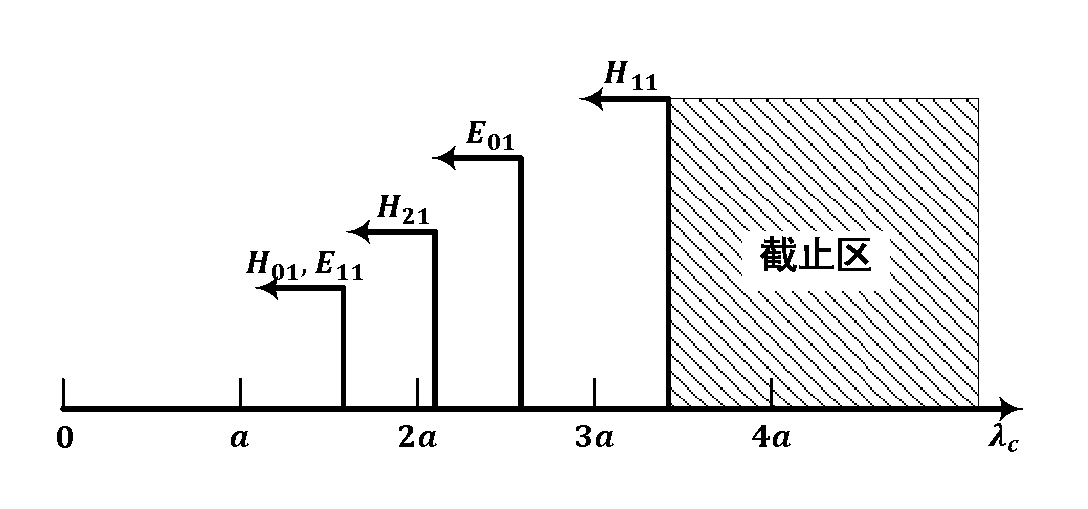
\includegraphics[width=10cm]{Cha6//fig6-20.pdf}
        \caption{圆波导的截止与传播区域}
    \end{figure}
\end{frame}

\begin{frame}{圆波导——简并}
    \begin{enumerate}
        \resume
        \item 圆波导的两种简并\\
              \begin{itemize}
                  \item 极化简并——即$\sin m\varphi$和$\cos m\varphi$两种,相互旋转$90^{\circ}$ \\
                        \footnotesize{圆波导波型的极化简并,使得传输不稳定,这是圆波导应用受到限制的主要原因。}
                  \item 另一种简并\\
                        \footnotesize{
                        $E_{1n}和H_{0n}$截止波长$\lambda_c$相同\\
                        $Bessel$函数有递推公式:\\
                        $xJ_n^{'}+nJ_n=xJ_{n+1}$,取$n=0$,有$J_0^{'}(x)=-J_1(x)$\\
                        因为$H_{0n}$是$J_0^{'}$的第$n$个根,$E_{1n}$是$J_1$的第$n$个根,很显然,这两类波型将发生简并。\\
                        和矩形波导不同,由于$TE,TM$截止波长的不同物理意义,$TE_{mn}$和$TM_{mn}$不发生简并
                        }
              \end{itemize}
        \item 波型指数$m,n$的含义\\
              $m$代表沿圆周$\varphi$分布的整驻波数\\
              $n$代表沿半径$r$分布场的最大值个数
    \end{enumerate}
\end{frame}

\begin{frame}{圆波导——三种主要波型}
    圆波导中三种主要波型,即$H_{11}$模,$H_{01}$模,$E_{01}$模。
    \begin{enumerate}
        \item 传输主模——$H_{11}$模\\
              在圆波导中,$H_{11}$模截止波长最长,$\lambda_c=3.412a$,是最低型模式也即传输主模。
              \saveenum
    \end{enumerate}
    \begin{figure}
        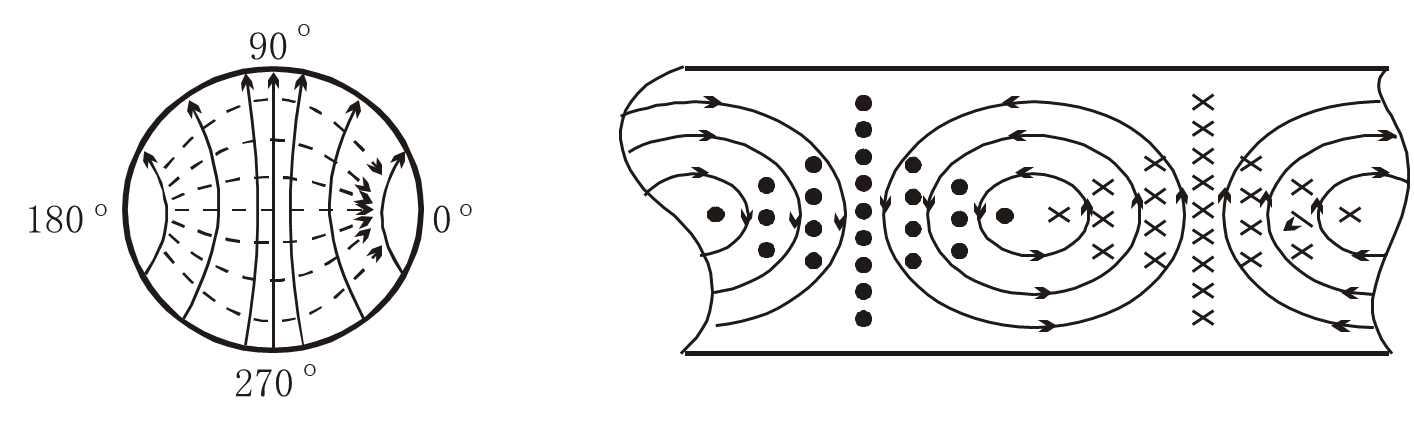
\includegraphics[width=10cm]{Cha6//fig6-21.png}
        \caption{圆波导$H_{11}$模}
    \end{figure}
\end{frame}

\begin{frame}{圆波导——三种主要波型}
    $H_{11}$模中的$m=1,n=1,u_{11}^{'}=1.841$
    \begin{align*}
        \begin{cases}
            E_z=0                                     \\
            H_z(r,\varphi,z)=H_{0}J_1\left(\dfrac{u_{11}^{'}}{a}r\right)
            \begin{matrix*}
                \cos \varphi\\
                \sin \varphi\\
            \end{matrix*}
            \mathrm{e}^{\mathrm{j}(\omega t-\beta z)} \\
            E_r=\pm\dfrac{\mathrm{j}\omega\mu a^2}{(u_{11}^{'})^2r}H_{0}J_1\left(\dfrac{u_{11}^{'}}{a}r\right)
            \begin{matrix*}
                \sin \varphi\\
                \cos \varphi\\
            \end{matrix*}
            \mathrm{e}^{\mathrm{j}(\omega t-\beta z)} \\
            E_{\varphi}=\dfrac{\mathrm{j}\omega\mu a}{u_{11}^{'}}H_{0}J_1^{'}\left(\dfrac{u_{11}^{'}}{a}r\right)
            \begin{matrix*}
                \cos \varphi\\
                \sin \varphi\\
            \end{matrix*}
            \mathrm{e}^{\mathrm{j}(\omega t-\beta z)} \\
            H_r=-\dfrac{\mathrm{j}\beta a}{u_{11}^{'}}H_{0}J_1^{'}\left(\dfrac{u_{11}^{'}}{a}r\right)
            \begin{matrix*}
                \cos \varphi\\
                \sin \varphi\\
            \end{matrix*}
            \mathrm{e}^{\mathrm{j}(\omega t-\beta z)} \\
            H_{\varphi}=\pm\dfrac{\mathrm{j}\beta a^2}{(u_{11}^{'})^2r}H_{0}J_1\left(\dfrac{u_{11}^{'}}{a}r\right)
            \begin{matrix*}
                \sin \varphi\\
                \cos \varphi\\
            \end{matrix*}
            \mathrm{e}^{\mathrm{j}(\omega t-\beta z)} \\
        \end{cases}
    \end{align*}
\end{frame}

\begin{frame}{圆波导——三种主要波型}
    \begin{table}
        \caption{$H_{11}$模的电场分布}
        \begin{tabular}{|c|c|c|}
            \hline
            m=1
             & {\makecell[c]{$\varphi=0^{\circ}\quad E_r=0$  \\$\varphi=90^{\circ}\quad E_r\to max$\\$\varphi=180^{\circ}\quad E_r=0$\\$\varphi=270^{\circ}\quad E_r\to -max$}}
             & \begin{minipage}[b]{0.3\columnwidth}
                   \centering
                   \raisebox{-.5\height}{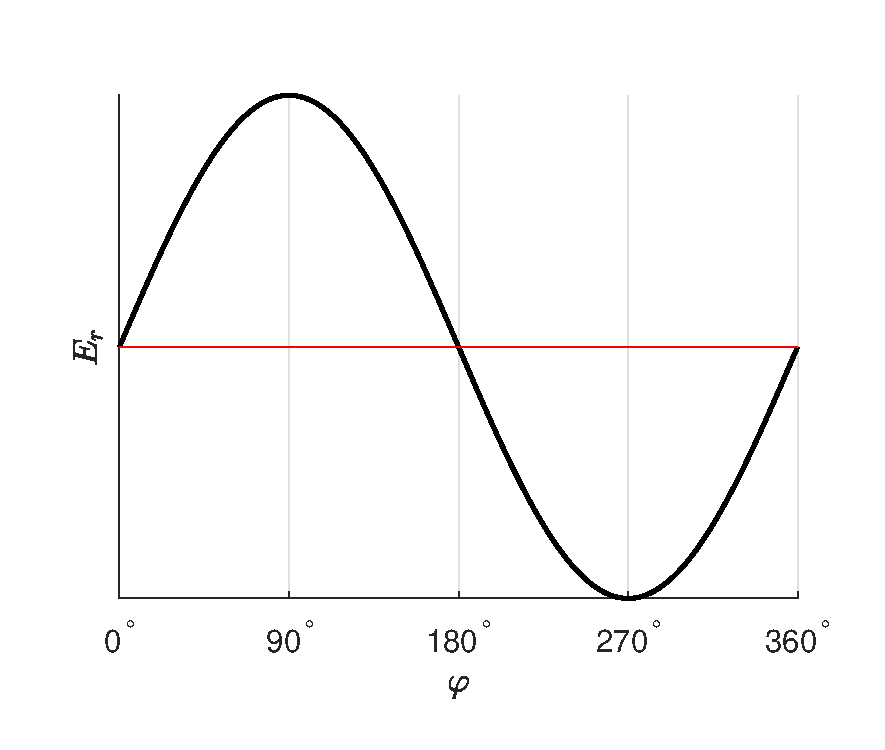
\includegraphics[width=4cm]{Cha6//fig6-22.pdf}}
               \end{minipage} \\
            \hline
            n=1
             & {\makecell[c]{$r=0\quad E_{\varphi}\to max$   \\$\downarrow$\\$r=a\quad E_{\varphi}=0$}}
             & \begin{minipage}[b]{0.3\columnwidth}
                   \centering
                   \raisebox{-.5\height}{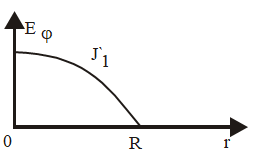
\includegraphics[width=4cm]{Cha6//fig6-23.png}}
               \end{minipage} \\
            \hline
        \end{tabular}
        %\label{table1}
    \end{table}
\end{frame}

\begin{frame}{圆波导——三种主要波型}
    $$\lambda_g=\lambda/\sqrt{1-(\lambda/3.412a)^2}$$
    可以注意到圆波导中$H_{11}$模与矩形波导中$TE_{10}$模极相似,因此微波工程中方圆过渡均采用$H_{11}$模。\\
    但是,$H_{11}$模有两种极化方向。因此一般很少用于微波传输线,而只用于微波元件。
    \begin{figure}
        \centering
        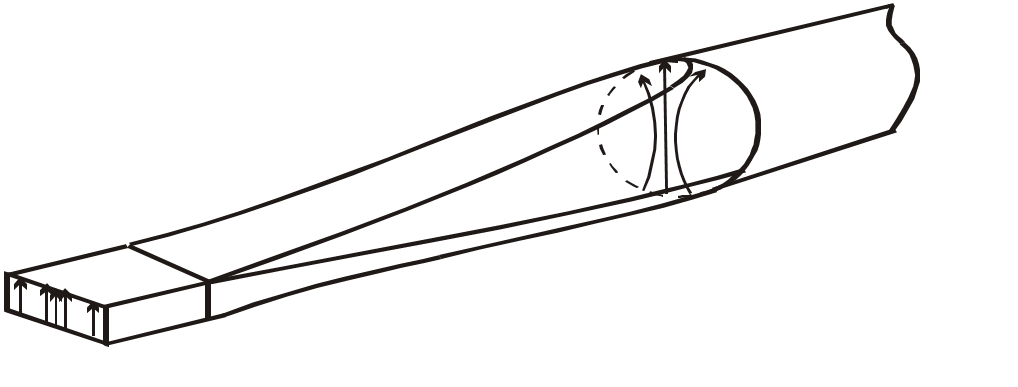
\includegraphics[width=9cm]{Cha6//fig6-24.png}
    \end{figure}
\end{frame}

\begin{frame}{圆波导——三种主要波型}
    \begin{enumerate}
        \resume
        \item 损耗最小模——$H_{01}$模\\
              $H_{01}$模常作为高$Q$谐振腔和远距离的毫米波传输线的工作模式。由于它是圆电模,也可作为连接元件和天线馈线系统的工作模式。
              由于它不是主模,用该模式作为工作模式时,必须设法抑制其他模式。
              \saveenum
    \end{enumerate}
    \begin{figure}
        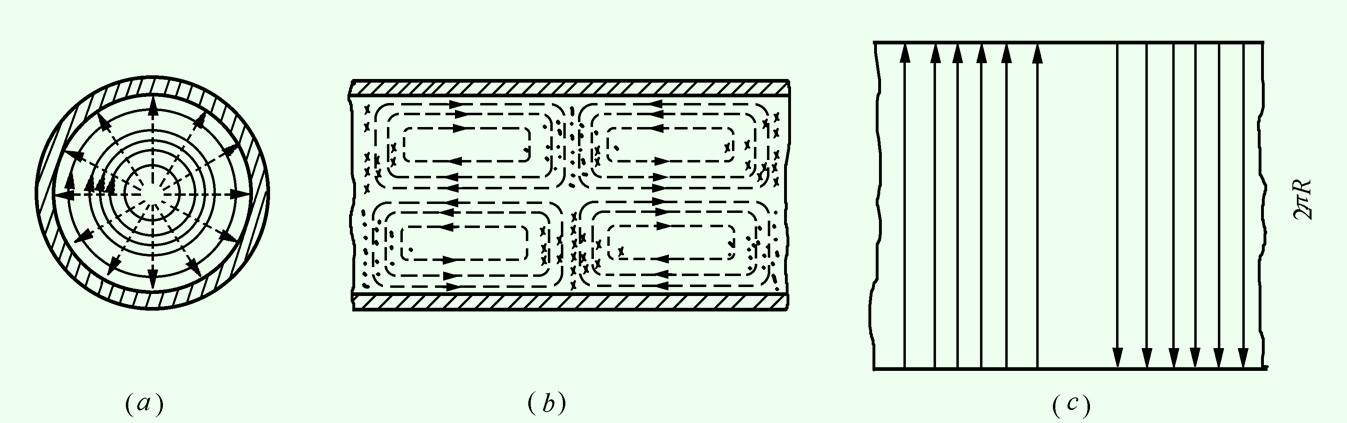
\includegraphics[width=8cm]{Cha6//fig6-25.png}
        \caption{圆波导$H_{01}$模}
    \end{figure}
\end{frame}

\begin{frame}{圆波导——三种主要波型}
    场分量
    \begin{align*}
        \begin{cases}
            E_{\varphi}=-\mathrm{j}\dfrac{\omega\mu a}{3.832}H_0J_1(3.832r/a)\mathrm{e}^{-\mathrm{j}\beta z} \\
            H_r=\mathrm{j}\dfrac{\beta a}{3.832}H_0J_1(3.832r/a)\mathrm{e}^{-\mathrm{j}\beta z}              \\
            H_z=H_0J_0(3.832r/a)\mathrm{e}^{-\mathrm{j}\beta z}
        \end{cases}
    \end{align*}
    截止波长
    $$\lambda_c=\frac{2\pi a}{3.832}=1.641a$$
    波导波长
    $$\lambda_g=\lambda/\sqrt{1-(\lambda/1.641a)^2}$$
\end{frame}

\begin{frame}{圆波导——三种主要波型}
    为了揭示$H_{01}$模的小衰减特点,让我们考察其壁电流
    $$\vec{J}_S=\hat{n}\times\vec{H}_z=-\hat{r}_0\times\vec{H}_z=\left\lvert\vec{H}_z\right\rvert\hat{\varphi} $$
    可见电流只有一个方向分量,衰减$\alpha$随$f$上升而下降
    $$\alpha_{H_{01}}=\frac{8.686R_s}{a\sqrt{\mu/\epsilon}}\frac{(\lambda/\lambda_c)^2}{\sqrt{1-(\lambda/\lambda_c)^2}}\quad dB/m$$
    作为比较
    $$\alpha_{H_{11}}=\frac{8.686R_s}{a\sqrt{\mu/\epsilon}}\frac{(\lambda/\lambda_c)^2+\color{red}{0.42}}{\sqrt{1-(\lambda/\lambda_c)^2}}\quad dB/m$$
    所以,$H_{01}$模可以做高$Q$谐振腔和毫米波远距离传输。
\end{frame}

\begin{frame}{圆波导——三种主要波型}
    \begin{enumerate}
        \resume
        \item 轴对称模——$E_{01}$模\\
              虽然$H_{01}$模和$E_{01}$模都是轴对称模,但$E_{01}$模是截止波长最长的模式。
    \end{enumerate}
    \begin{figure}
        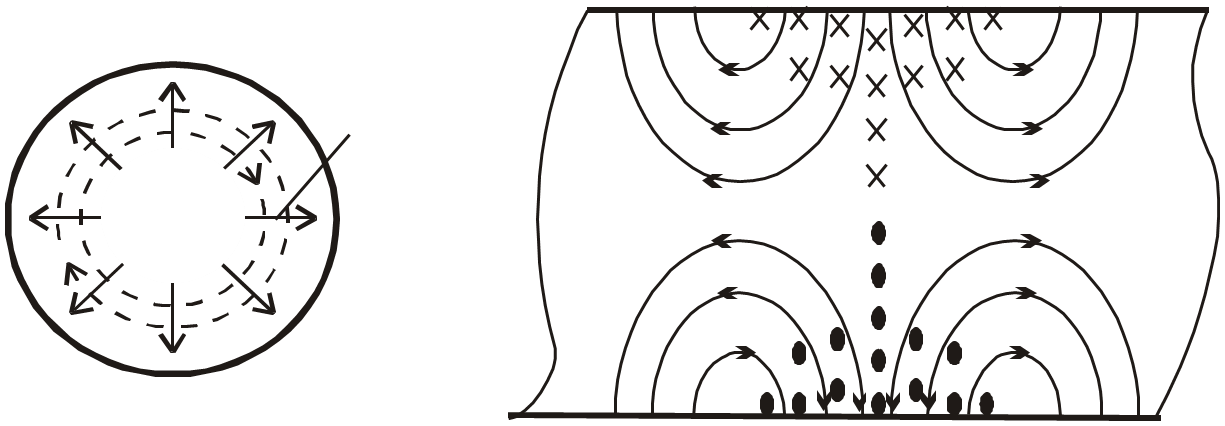
\includegraphics[width=8cm]{Cha6//fig6-26.png}
        \caption{圆波导中$E_{01}$模}
    \end{figure}
\end{frame}

\begin{frame}{圆波导——三种主要波型}
    $E_{01}$模的场分布如下图所示。图(a)表示横截面上的电磁场分布;图(b)表示纵剖面上的电磁场分布;图(c)为壁电流分布。
    \begin{figure}
        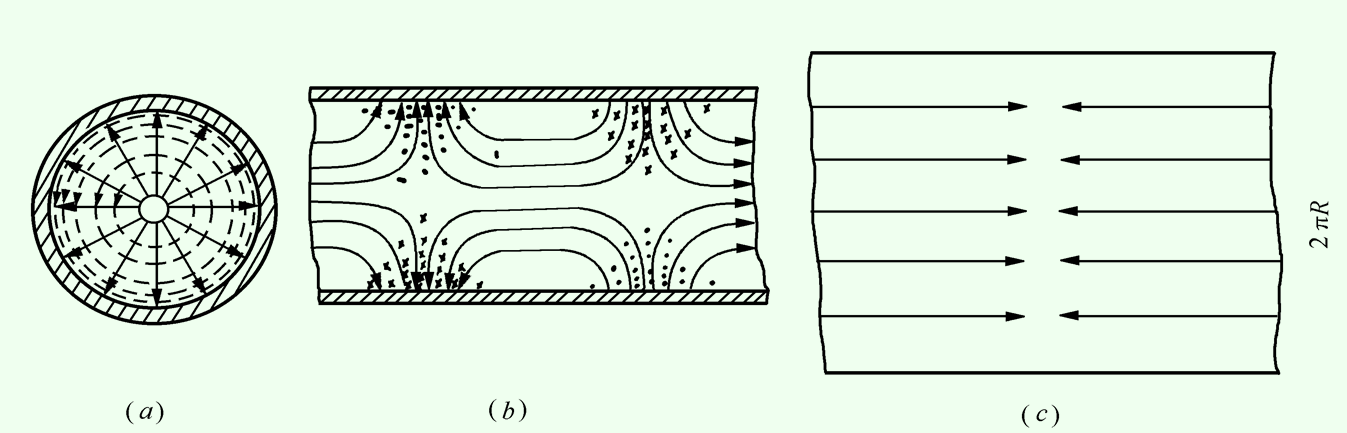
\includegraphics[width=8cm]{Cha6//fig6-27.png}
    \end{figure}
    $E_{01}$模适用于微波天线馈线旋转铰链的工作模式。由于它具有$E_z$分量,便于和电子交换能量,可作电子直线加速器的工作模式。但
    由于它的管壁电流具有纵向电流,故必须采用抗流结构的连接方式。
\end{frame}

\begin{frame}{圆波导——三种主要波型}
    场分量
    \begin{gather*}
        \begin{cases}
            E_z(r,\varphi,z)=E_0J_0\left(\dfrac{u_{01}}{a}r\right)\mathrm{e}^{-\mathrm{j}\beta z}                          \\
            E_r=-\dfrac{\mathrm{j}\beta a}{u_{01}}E_0J_0^{'}\left(\dfrac{u_{01}}{a}r\right)\mathrm{e}^{-\mathrm{j}\beta z} \\
            H_{\varphi}=-\dfrac{\mathrm{j}\omega\epsilon a}{u_{01}}E_0J_0^{'}\left(\dfrac{u_{01}}{a}r\right)\mathrm{e}^{-\mathrm{j}\beta z}
        \end{cases}\\
        u_{01}=2.405,\lambda_c=2.62a\\
        \lambda_g=\lambda/\sqrt{1-(\lambda/2.62a)^2}
    \end{gather*}
\end{frame}

\begin{frame}{圆波导——三种主要波型}
    由于$E_{01}$模的特点,常做雷达的旋转关节,如下图
    \begin{figure}
        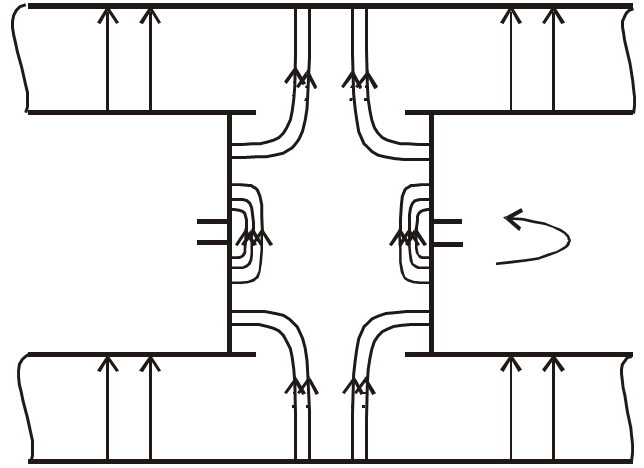
\includegraphics[width=5cm]{Cha6//fig6-28.png}
        \caption{旋转关节(Ratation Junction)}
    \end{figure}
\end{frame}

\begin{frame}{圆波导——波型设计}
    \begin{table}
        \begin{threeparttable}[b]
            \caption{圆波导波型设计}
            \setlength{\tabcolsep}{8mm}{
                \begin{tabular}{|c|c|c|}
                    \hline
                    $H_{11}$模
                     & {\makecell[c]{$\lambda_{cE_{01}}<\lambda<\lambda_{cH_{11}}$   \\$2.62a<\lambda<3.41a$}}
                     & {\makecell[c]{$\dfrac{\lambda}{3.41}<a<\dfrac{\lambda}{2.62}$ \\一般选$a\approx \dfrac{1}{3}\lambda$}}\\
                    \hline
                    $E_{01}$模
                     & {\makecell[c]{$\lambda_{cH_{21}}<\lambda<\lambda_{cE_{01}}$   \\$2.06a<\lambda<2.62a$}}
                     & $\dfrac{\lambda}{2.62}<a<\dfrac{\lambda}{2.06}$               \\
                    \hline
                    $H_{01}$模
                     & {\makecell[c]{$\lambda_{cE_{21}}<\lambda<\lambda_{cH_{01}}$   \\$1.22a<\lambda<1.64a$}}
                     & $\dfrac{\lambda}{1.64}<a<\dfrac{\lambda}{1.22}$               \\
                    \hline
                \end{tabular}
            }
        \end{threeparttable}
    \end{table}
\end{frame}

\subsection{同轴线}
\begin{frame}{同轴线}
    同轴线是一种双导体传输线。内外导体之间填充高频介质。
    \begin{figure}
        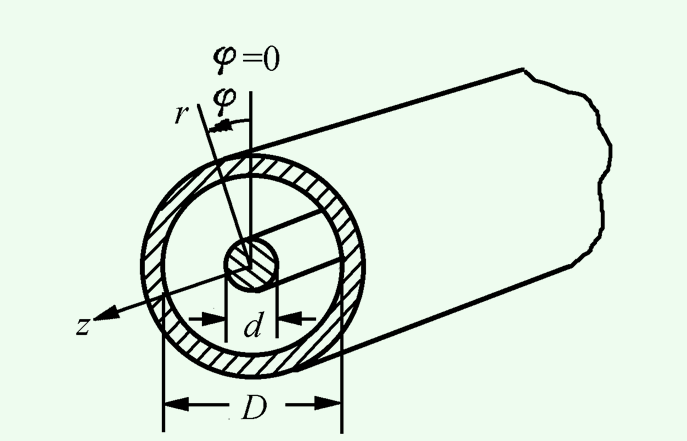
\includegraphics[width=6cm]{Cha6//fig6-29.png}
    \end{figure}
    在同轴线中既可传输无色散的$TEM$波,也可能存在有色散的$TE$和$TM$波。
\end{frame}

\begin{frame}{同轴线——传输主模TEM}
    \begin{enumerate}
        \item $TEM$模的场分量和场结构
        \begin{gather*}
            E_z=H_z=0\\
            \vec{E}(r,\varphi,z)=\vec{E}_t(r,\varphi,z)=\vec{E}_{0t}(r,\varphi)\mathrm{e}^{-\mathrm{j}\beta z}
        \end{gather*}
        由
        $$\nabla_t\times \vec{E}_t=-\mathrm{j}\omega\mu\hat{z}H_z=0$$
        引入势函数$\color{red}{\Phi(r,\varphi)\qquad \vec{E}_{0t}(r,\varphi)=-\nabla_t\Phi(r,\varphi)}$
        $$\vec{E}(r,\varphi,z)=\vec{E}_{0t}(r,\varphi)\mathrm{e}^{-\mathrm{j}\beta z}=-\nabla_t\Phi(r,\varphi)\mathrm{e}^{-\mathrm{j}\beta z}$$
        又$\nabla\cdot \vec{E}_t=0$
        $$\color{red}{\nabla_t^2\Phi(r,\varphi)=0}$$
        \saveenum
    \end{enumerate}
\end{frame}

\begin{frame}{同轴线——传输主模TEM}
    势满足拉普拉斯方程
    $$\frac{1}{r}\frac{\partial}{\partial r}\left(r\frac{\partial\Phi(r,\varphi)}{\partial r}\right)+\frac{1}{r^2}\frac{\partial^2\Phi(r,\varphi)}{\partial\varphi^2}=0$$
    \begin{columns}
        \begin{column}{0.5\linewidth}
            边界条件:\\
            \begin{align*}
                &\Phi(a,\varphi)=V_0\\
                &\Phi(b,\varphi)=0
            \end{align*}
            令$\Phi(r,\varphi)=R(r)F(\varphi)$
        \end{column}
        \begin{column}{0.5\linewidth}
            \begin{figure}
                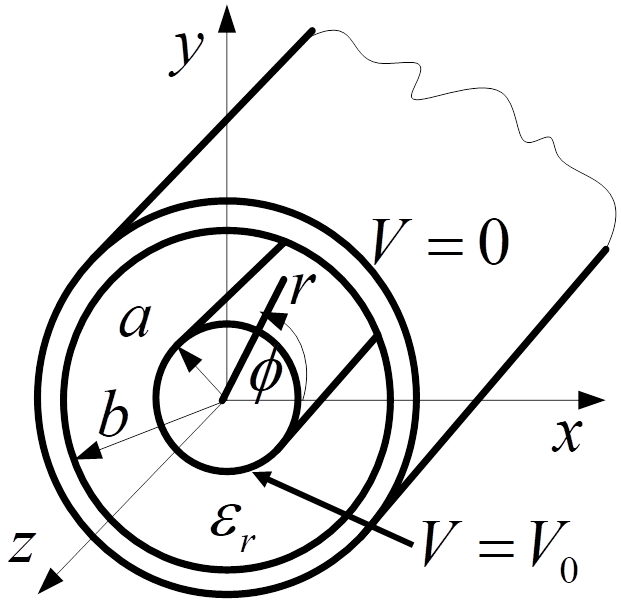
\includegraphics[width=4cm]{Cha6//fig6-30.png}
            \end{figure}
        \end{column}
    \end{columns}
\end{frame}

\begin{frame}{同轴线——传输主模TEM}

\end{frame}

\begin{frame}{同轴线——传输主模TEM}

\end{frame}

\begin{frame}{同轴线——传输主模TEM}

\end{frame}

\begin{frame}{同轴线——传输主模TEM}

\end{frame}

\begin{frame}{同轴线——传输主模TEM}

\end{frame}

\begin{frame}{同轴线}

\end{frame}

\begin{frame}{同轴线}

\end{frame}

\begin{frame}{同轴线}

\end{frame}

\begin{frame}{同轴线}

\end{frame}

\begin{frame}{同轴线}

\end{frame}

\subsection{平面传输线}
\begin{frame}{平面传输线}
    上世纪六十年代以来,在微波工程和微波技术上,出现了一次不小的革命,即所谓MIC(Microwave Integrated Circuit)微波集成电路——HMIC、MMIC。其特色是体积小、功能多、频带宽,但承受功率小。因此被广泛应用于接收机和小功率元件中,并都传输TEM波。\\
    作为这一革命的“过渡人物”是带状线(Stripline)。它可以看作是同轴线的变形。
\end{frame}

